%%%%%%%%%%%%%%%%%%%%%%%%%%%%%%%%%%%%%%%%%
% Masters/Doctoral Thesis
%
% %%%%% IMPORTANT %%%%%
% 1) Edit Front/vars.tex
% 2) Compile Front/main.tex
% 3) Edit vars.tex
% 4) Edit precontent.tex
%
% BEFORE ANYTHING ELSE
% You can also set some interesting stuff in the preamble.tex file
% If you know what you're doing.
%%%%%%%%%%%%%%%%%%%%%%%%%%%%%%%%%%%%%%%%%

% The default font size and two-sided printing
% For a one-sided printing change the flag "twoside" to "oneside"
\documentclass[11pt, twoside, table,xcdraw]{Thesis}


%-------------------------------------------------------------------------
%   PREAMBLE AND SETTINGS
%-------------------------------------------------------------------------
% Add the preamble. You can change various settings in here
%-------------------------------------------------------------------------
%	PACKAGES AND OTHER DOCUMENT CONFIGURATIONS
%-------------------------------------------------------------------------

% Include pdf pages in the document
% Necessary to include the front pages (cover and etc.)
\usepackage{pdfpages}

% Fix top page geometry on long titles
\setlength{\headheight}{14pt}  %Try fix error

% Language hyphenation and typographical rules
\usepackage[portuguese,english]{babel}
%Custom hyphenization
\hyphenation{Py-thon}
\hyphenation{Ju-py-ter}
\hyphenation{Ma-the-ma-ti-ca}

% Inline quotes
% added for \begin{displayquote}
\usepackage[autostyle]{csquotes}

% Bibliography setup
% Use the natbib reference package - read up on this to edit the reference
% style; if you want text (e.g. Smith et al., 2012) for the in-text references
% (instead of numbers), remove 'numbers'
\usepackage[square, numbers, comma, sort&compress]{natbib}
\bibliographystyle{IEEEtranN}  % I actually quite like this one
% \bibliographystyle{apsrev4-1-etal} % With emphasized titles. ORIGINAL
% Prevent that the first citation is in the ToC
\usepackage{notoccite}

% Interesting float placements (like 'H') and custom float types
\usepackage{float}
% Text wrapped around pictures
% https://pt.sharelatex.com/learn/Wrapping_text_around_figures
\usepackage{wrapfig}
% Force float barriers, use as \FloatBarrier
\usepackage[section]{placeins}
% Place floats *above* footnotes
\usepackage[bottom, perpage, symbol]{footmisc}
% Set default float placement
\makeatletter
\renewcommand{\fps@figure}{tbph}
\renewcommand{\fps@table}{tbph}
\makeatother

% Pretty colours
\usepackage{xcolor}
% \usepackage{color} % Deprecated by xcolor

% SVGs with Inkscape and PDF+LaTeX
% https://tex.stackexchange.com/questions/473994/svg-and-inkscape
\usepackage[inkscapearea=page]{svg}
% Specifies the directory where vector are stored
\svgpath{{Svgs/}}

% Graphics stuff
\usepackage{graphicx}  % invoked by svg
\usepackage{tikz-cd}
\usetikzlibrary{babel}
% Specifies the directory where pictures are stored
\graphicspath{{Figures/}}

% For sub-figures and stuff
\usepackage{caption}
\usepackage{subcaption}

% Math stuff
\usepackage{amsmath} % Interesting environments
\usepackage{amssymb} % Interesting symbols
\usepackage{mathrsfs}
\usepackage{commath} % Interesting macros
\usepackage{braket} % Dirac bra-ket and set notations
\usepackage{mathpazo} % Math font (palatino for Computer Modern on math)
\usepackage{mathtools} % Mathematical tools to use with amsmath
\setstretch{1.5}
% Math alphabet
\DeclareMathAlphabet{\pazocal}{OMS}{zplm}{m}{n}
\newcommand{\Sa}{\pazocal{S}}
\newcommand{\Ua}{\pazocal{U}}
\newcommand{\Ha}{\pazocal{H}}
\newcommand{\Fa}{\pazocal{F}}
\newcommand{\Ia}{\pazocal{I}}
\newcommand{\Ea}{\pazocal{E}}
\newcommand{\ja}{\pazocal{J}}
%Custom math operators
\DeclareMathOperator*{\meshgrid}{meshgrid}
\newcommand{\subgen}[1]{\langle #1 \rangle}
\newcommand{\card}[1]{| #1 |}
\newcommand{\nsub}{\triangleleft}
\newcommand{\cmpl}[1]{\overline{ #1 }}
\newcommand{\dt}[2]{(#1)_{#2}}
\newcommand{\soc}[1]{soc {(#1)}}
\newcommand{\diag}[1]{diag({#1})}
\newcommand{\Mi}[1][i]{M_{#1}}
\newcommand{\dl}[0]{\dot{l}}
\newcommand{\core}[1]{core({#1})}
\newcommand{\aut}[1]{Aut\, {#1}}
\newcommand{\inn}[1]{Inn\, {#1}}
% Floor and ceiling of numbers
\DeclarePairedDelimiter\ceil{\lceil}{\rceil}
\DeclarePairedDelimiter\floor{\lfloor}{\rfloor}
% Notation variables
\newcommand{\dd}{\mathrm{d}}

% Units and numbers in text
\usepackage{siunitx}
\DeclareSIUnit\baud{Bd} % Baud

% Reimplementation of and extensions to LaTeX verbatim
\usepackage{verbatim} %added for \begin{comment}

% Fancy chapter start quotes
\usepackage{epigraph, varwidth}
\input{epigraphoverload}

% Use more than one optional parameter in a new commands
\usepackage{xargs}

% Code listings
\usepackage{listings}
% Colors for the listing
\definecolor{dkgreen}{rgb}{0,0.6,0}
\definecolor{gray}{rgb}{0.5,0.5,0.5}
\definecolor{mauve}{rgb}{0.58,0,0.82}
\definecolor{codegreen}{rgb}{0,0.6,0}
\definecolor{codegray}{rgb}{0.5,0.5,0.5}
\definecolor{codepurple}{rgb}{0.58,0,0.82}
\definecolor{backcolour}{rgb}{0.95,0.95,0.92}
\definecolor{orange}{RGB}{255,127,0}
% Python style for code blocks
\lstdefinestyle{Python}{
        language=Python,
         numberstyle=\small,
         stepnumber=2,
         numbersep=10pt,
         basicstyle={\small\ttfamily},
         keywordstyle    = \color{blue},
         commentstyle    = \color{red}\ttfamily,
         stringstyle=\color{orange},
         tabsize=2,
         columns=fullflexible,
         backgroundcolor=\color{backcolour},
         frame=none,
         numbers=left,
         aboveskip=5mm,
         belowskip=5mm,
         breaklines=true
}

% Algorithmicx provides a flexible, yet easy to use, way for inserting good
% looking pseudocode or source code in your papers.
\usepackage{algorithmicx}

% Hyperref and Backref
% backref makes the bibliography say where the entry was cited.
% For the print version of the thesis you might wanna set all colors to back
\usepackage{hyperref}
\usepackage[hyperpageref]{backref}
\hypersetup{colorlinks, citecolor=blue, urlcolor=blue,
        linkcolor=blue, breaklinks=true, hypertexnames=true}
\renewcommand*{\backref}[1]{}
\renewcommand*{\backrefalt}[4]{%
    \ifcase #1%
          \or [Cited on page~#2.]%
          \else [Cited on pages~#2.]%
    \fi%
    }
% Interesting URL breakings
\usepackage{url}
\def\UrlBreaks{\do\/\do-\do\&\do.\do:}

% Variants of \fbox and other games with boxes
\usepackage{fancybox}

% LaTeX default text is fully-justified, but often left-justified text may be a
% more suitable format. This left-alignment can be easily accomplished by
% importing the ragged2e package.
\usepackage{ragged2e}

% Create tabular cells spanning multiple rows
\usepackage{multirow}

% Changes bullet points marker
\renewcommand{\labelitemi}{\(\bullet\)}

% Notes on the documents
% https://tex.stackexchange.com/questions/9796/how-to-add-todo-notes
% https://tex.stackexchange.com/questions/316220/todo-commentsnot-include-and-left-align
% Examples:
% \unsure{Is this correct?}, \change{Change this!},
% \info{This can help me in chapter seven!}
% \improvement{This really needs to be improved!\\ What was I thinking?!}
% \thiswillnotshow{This is hidden since option `disable' is chosen!}
% WARNING: It eliminates whitespaces in front of it.
% You can add trailing {} to avoid.

\usepackage[colorinlistoftodos,
    prependcaption,
    textsize=tiny,
    textwidth=2cm]
        {todonotes}
% You can add:
% \setlength{\marginparwidth}{3cm}\reversemarginpar
% before \todo on each command for a different effect
\newcommandx{\unsure}[2][1=]{
    % \setlength{\marginparwidth}{3cm}\reversemarginpar
    \todo[linecolor=red,backgroundcolor=red!25,bordercolor=red,#1]{#2}
    }
\newcommandx{\change}[2][1=]{
    % \setlength{\marginparwidth}{3cm}\reversemarginpar
    \todo[linecolor=blue,backgroundcolor=blue!25,bordercolor=blue,#1]{#2}
    }
\newcommandx{\info}[2][1=]{
    % \setlength{\marginparwidth}{3cm}\reversemarginpar
    \todo[linecolor=green,backgroundcolor=green!25,bordercolor=green,#1]{#2}
    }
\newcommandx{\improvement}[2][1=]{
    % \setlength{\marginparwidth}{3cm}\reversemarginpar
    \todo[linecolor=yellow,backgroundcolor=yellow!25,bordercolor=yellow,#1]{#2}
    }
\newcommandx{\thiswillnotshow}[2][1=]{\todo[disable,#1]{#2}}


% Thesis settings. THIS IS VERY IMPORTANT YOU CHANGE
% !TEX root = main.tex

%-------------------------------------------------------------------------
%	PARAMETERS FOR FCUP THESIS TITLEPAGES/BOOK COVER
%-------------------------------------------------------------------------

% THESIS TYPEs:
% - msc (Master of Sciences)
% - phd (Doctor of Philosophy)
\thesistype{msc}

% Book spine width (CAREFUL: MIN 8mm)
\spinewidth{10mm}

% Thesis front title
\fronttitle{On the minimal number of generators of a finite group}

% Front title spacing multiplier
% NOTE: you may want to adjust this value to 1.15/1.20 after changing to your
% thesis title
\titlespacing{1.15}

% Book spine title
\spinetitle{Spine Title}

% Author name
\authorname[mailto:up201905843@fc.up.pt]{Diogo Santos}

% Affiliation number 2
% USAGE: \otheraffiliation[url]{relative/path/to/logo}{INITIAL}{University name}
%\otheraffiliation[http://uni2.pt]{logos/logo2}{UNI2}{Universidade/Faculdade 2}

% Affiliation number 3
% USAGE: \extraaffiliation[url]{relative/path/to/logo}{INITIAL}{University name}
%\extraaffiliation[http://uni3.pt]{logos/logo3}{UNI3}{Universidade/Faculdade 3}

% Degree name
\degreename{Mestrado em Matemática}

% Field of science
\sciencefield{Matemática}

% Department name
\department[https://matematica.fc.up.pt/en/department]{Departamento de Matemática}

% Supervisor info
% Supervisor name
\supervisor[mailto:claude.marion@fc.up.pt]{Prof. Dr. Claude Marion}
% Supervisor name position/Category (comment out to hide this field)
%\supervisorposition{Categoria} %
% Supervisor university/faculty
\supervisoraffiliation[]{Faculdade de Ciências}
% Supervisor secondary affiliation
%\supervisoraffiliation[]{Instituto de Engenharia de Sistemas e Computadores,
% Tecnologia e Ciência}

% Cosupervisor info ----- Comment out if not needed
% Cosupervisor name
%\cosupervisor[mailto:example@fc.up.pt]{Prof. Dr. Galileu Galilei}
% Cosupervisor name position/Category (comment out to hide this field)
%\cosupervisorposition{Categoria}
% Supervisor university/faculty
%\cosupervisoraffiliation[]{Faculdade de Ciências}

% ------------------


%-------------------------------------------------------------------------
%	DOCUMENT
%-------------------------------------------------------------------------

\begin{document}

% Start counting pages in an unused scheme to fix backref
\pagenumbering{Alph}

% Includes the front pages (cover and etc.)
\pagestyle{empty}
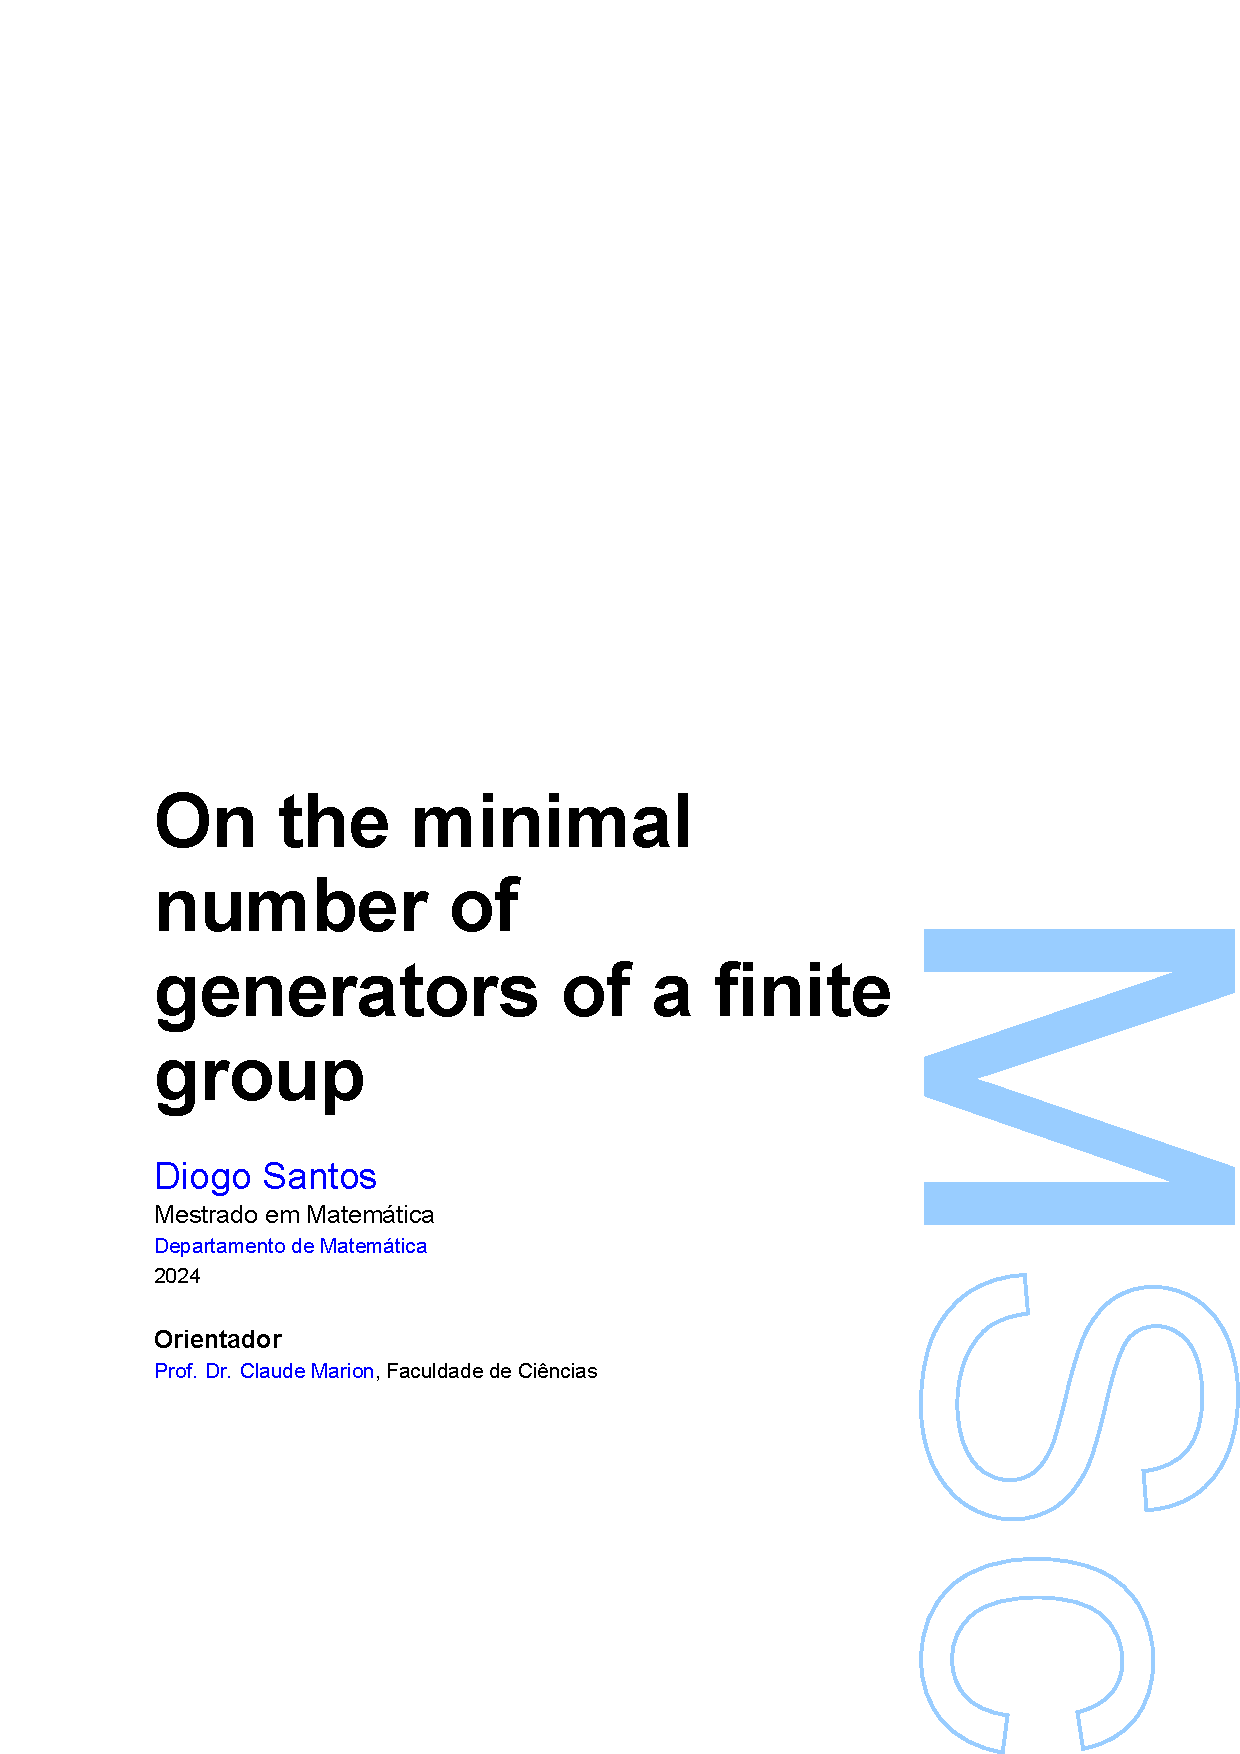
\includepdf[pages={1},pagecommand={},scale=1]{Front/main}
\cleardoublepage
\includepdf[pages={2},pagecommand={},scale=1]{Front/main}
\cleardoublepage
\pagestyle{fancy}

% Use roman page numbering style (i, ii, iii, iv...) for the pre-content pages
\frontmatter

% Title page
\maketitle

% Edit this file!

%-------------------------------------------------------------------------
%	QUOTATION PAGE
%-------------------------------------------------------------------------
%%\quotepage{Matt Smith as \emph{The Doctor}, written by Matthew Graham}
%{
%	Mais je n’ai pas le temps et mes idées ne sont pas encore bien développées sur ce terrain qui est immense.
%}
%
%-------------------------------------------------------------------------
%	ACKNOWLEDGEMENTS PAGE
%-------------------------------------------------------------------------
\begin{acknowledgements}

	I would like to express my gratitude to my supervisor, Professor Claude Marion, for his valuable guidance and expertise, as well as for sparking my interest in this fascinating subject.

\end{acknowledgements}

\addvspacetoc{0.3cm} % Add a gap in the Contents, for aesthetics


%-------------------------------------------------------------------------
%	ABSTRACT PAGE
%-------------------------------------------------------------------------
\begin{abstract}
	A generalization of a structure Theorem is provided for finite groups with the property that, for some positive integer $m$ every proper quotient can be generated by $m$ elements but the group itself cannot. 
	Furthermore, detailed proofs were provided for the calculation of the integer $k$ of the groups $L_k$.
\end{abstract}

%-------------------------------------------------------------------------
%	ABSTRACT PAGE (PORTUGUESE)
%-------------------------------------------------------------------------
%\begin{abstract}[
%	thesistitle={Titulo da Tese em Portugês},
%	title={Resumo},
%	degree={Mestrado Integrado em Engenharia Física},
%	nameconnector={por}]
%\begin{otherlanguage}{portuguese}
%
%Este tese é sobre alguma coisa
%
%\end{otherlanguage}
%\end{abstract}

%-------------------------------------------------------------------------
%	LIST OF CONTENTS/FIGURES/TABLES
%-------------------------------------------------------------------------

\addvspacetoc{0.3cm}

\tableofcontents % Write out the Table of Contents

%\listoffigures % Write out the List of Figures

%\listoftables % Write out the List of Tables

%\addvspacetoc{0.3cm}

%-------------------------------------------------------------------------
%	PHYSICAL CONSTANTS/OTHER DEFINITIONS
%-------------------------------------------------------------------------

%\begin{listofcontants}
%	\const{My little ponny test of magical rainbow}{$mn/mp$}
%    {$2.997\ 924\ 58\times10^{8}\ \mbox{ms}^{-\mbox{s}}$}
%   \const{Vaccuum permeability test of magical rainbow for a specific case of
%   condensed matter physics}
%   {$\epsilon_0$}{$2.997\ 924\ 58\times10^{8}\ \mbox{ms}^{-\mbox{s}}$}
%	\const{Speed of Light test of magical rainbow}{$c$}
%    {$2.997\ 924\ 58\times10^{8}\ \mbox{ms}^{-\mbox{s}}$}
%\end{listofcontants}


%-------------------------------------------------------------------------
%	SYMBOLS
%-------------------------------------------------------------------------

%\begin{listofsymbols}
%	\symb{$F_{\mu\nu}$}{Maxwell tensor}{F}
%	\symb{$a$}{distance}{m}
%	\\
%	\symb{$\omega$}{angular frequency}{rads$^{-1}$}
%\end{listofsymbols}


%-------------------------------------------------------------------------
%	NOTATION
%-------------------------------------------------------------------------

% \newcommand\notationname{Notation and Conventions}
% \addtotoc{\notationname}
% \fancyhead[LO]{\textsc{\notationname}}

% \input{Notation}



%-------------------------------------------------------------------------
%	ABBREVIATIONS
%-------------------------------------------------------------------------

%\begin{glossary}
%	\abbrev{QM}{Quantum Mechanics}
%\end{glossary}


%-------------------------------------------------------------------------
%	DEDICATORY
%-------------------------------------------------------------------------

%\begin{dedicatory}
%	This thesis is dedicated to my family, for their love and support.
%\end{dedicatory}



%-------------------------------------------------------------------------
%	THESIS CONTENT - CHAPTERS
%-------------------------------------------------------------------------

\addvspacetoc{0.3cm}

% Begin numeric (1,2,3...) page numbering
\mainmatter

\pagestyle{fancy}
\renewcommand{\chaptermark}[1]{\markboth{\thechapter. \textsc{#1}}{}}
\fancyhead[LO]{\leftmark}

%%% -----------  ADD CHAPTERS HERE ------------------ %%%

\chapter*{Introduction}
\addcontentsline{toc}{section}{Introduction}
One of the questions in finite group theory is to determine the minimal number of generators of a finite group.

For a finite group $H$, the minimal number of generators $d(H) = min\left\{\card{X}|\subgen{X} = H \right\}$ always exists. This is so because $H$ is always generated by itself, a finite set. On the other hand there are infinite groups that do not have a minimal number of generators. One such example is $\mathbb{Z}^{\mathbb{N}}$, the infinite direct product of copies of $\mathbb{Z}$.

It is not generally true that given a group $H$ and a subgroup $K \le H$, $d(K) \le d(H)$. 
In fact, the evidence suggests that there is very little we can say in general about the relationship between $d(H)$ and $d(K)$ for some subgroup $K$ of $H$. By Cayley's Theorem \cite[p.~52]{RotmanITG}, every finite group can be embedded in a symmetric group $S_n$, given a large enough integer $n$. It is also well known that $d(S_n) = 2$ \cite[p.~24]{RotmanITG}. In addition there are finite groups with any minimal number of generators. The group $(\mathbb{Z}_2)^d$, the direct product of $d$ copies of the additive group of integers modulo $2$, is generated by $d$ elements for any positive integer $d$. Thus, any result about the minimal number of generators of subgroups has to account for the fact that any finite group can be embedded in a finite group generated by two elements.

On the other hand, it is easily verifiable that for any $N \nsub H$, $d(H/N) \le d(H)$. 
This is so as the generators $h_1,\ldots,h_n$ of $H$, induce generators of $H/N$, namely $h_1N, \ldots , h_nN$.


It has been shown \cite{AschbacherSAFCG} that two generators are sufficient to generate any finite simple group.
With our current understanding, we can already break down the problem and make meaningful progress in addressing the issue for generic finite groups.

In fact for a generic finite group $H$, either $d(H) > d(H/K)$ for all non-trivial subgroups $K \nsub H$ or there is some non-trivial $K \nsub H$ such that $d(H) = d(H/K)$. In the second case the problem is reduced to that of determining the minimal number of generators of $H/K$, usually an easier task since $H/K$ has a smaller order than that of $H$. Now the group $H/K$ can again have a non-trivial normal subgroup $L/K$ such that $d(H/K) = d((H/K)/(L/K))$ and if that is the case the problem can again be simplified. Proceeding in this manner, the problem of determining the minimal number of generators of a generic finite group $H$ can be reduced to the problem of finding the minimal number of generators of finite groups $K$ which are generated by more elements than any of its proper non-trivial quotients i.e the first case.

Spectacular results regarding this problem were presented in \cite{DallaVoltaFGNMGAPQ}. These results rely on advanced group theory concepts and, although extremely valuable, have some omissions in their explanation, which this dissertation aims to fill.

\chapter{Preliminaries}

This section aims at laying out the necessary prerequisites for the results that follow in this dissertation.
Basic group theory concepts such as the notions of group, subgroup, normal subgroup, group action and Sylow subgroups are assumed.

\section{Normal closure}

Similar to what is done for subgroups (for example in \cite{RotmanITG}) it is possible to define normal subgroups generated by a set.

\begin{definition}
    Let $G$ be a group. If $x,y \in G$ we will denote the element $yxy^{-1}$ by $x^{y}$.
\end{definition}

\begin{theorem}
    \label{gnsub}
    The intersection of any family of normal subgroups of a group $G$ is again a normal subgroup of $G$.
\end{theorem}

\begin{proof}
    Let $\left\{ S_i |i \in I \right\}$ be a family of subgroups of $G$. It is well known that $\bigcap_{i \in I} S_i$ is a subgroup. Furthermore for any $i \in I$ and $g \in G$, $gS_ig^{-1} = S_i$ and thus $g(\bigcap_{i \in I} S_i)g^{-1} = \bigcap_{i \in I} gS_ig^{-1} = \bigcap_{i \in I} S_i$.  
\end{proof}

\begin{theorem}
    If $X$ is a subset of a group $G$, then there is a \textbf{smallest} normal subgroup $H$ of $G$ containing $X$; that is if $X \subseteq S$ and $S \nsub G$, then $H \nsub S$.   
\end{theorem}

\begin{proof}
    There are normal subgroups of $G$ containing $X$; for example, $G$ itself is normal and contains $X$; let us define $H$ as the intersection of all the normal subgroups of $G$ which contain $X$. Also let us note that $H$ is a normal subgroup, by Theorem \ref{gnsub}, and $X \subseteq H$. If $S \nsub G$ and $X \subseteq S$, then $S$ is one of the subgroups of $G$ being intersected to form $H$; hence, $H \le S$, and so $H$ is the smallest such subgroup.
\end{proof}

\begin{definition}
    If $X$ is a subset of a group $G$, then the smallest normal subgroup of $G$ containing $X$, denoted by $\subgen{X}_G$, is called the \textbf{normal closure of $X$}. If $X$ is a finite set, say $X = \{a_1, \ldots , a_n \}$ then we write $\subgen{X}_G = \subgen{a_1, \ldots , a_n}_G$ instead of $\subgen{X}_G = \subgen{\left\{a_1, \ldots , a_n\right\}}_G$.
\end{definition}

\begin{theorem}
    Let $G$ be a group and $X$ a subset of $G$. The normal closure of $X$ is the group $W = \subgen{\left\{gxg^{-1}|g \in G, x \in X\right\}}$. 
\end{theorem}

\begin{proof}
    If $y \in W$ then $y$ is a word on elements of $\left\{gxg^{-1}|g \in G, x \in X\right\}$, say $y = w_1\ldots w_n$. Obviously for any $g \in G$, $gyg^{-1} =gw_1g^{-1}\ldots gw_ng^{-1}$ is also a word on elements of $\left\{gxg^{-1}|g \in G, x \in X\right\}$. We have thus proved that $W$ is a normal subgroup of $G$ and since $\subgen{X}_G$ is the smallest normal subgroup that contains $X$, we have that $\subgen{X}_G \subseteq W$.
    
    On the other hand since $\subgen{X}_G$ is a normal subgroup of $G$ that contains $X$, it obviously contains $gxg^{-1}$ for any $x \in X$, $g \in G$. Thus $W \subseteq \subgen{X}_G$.
\end{proof}

\section{Semidirect Products}

\begin{definition}
    Let $K$ be a subgroup of a group $G$. A subgroup $Q \subseteq G$ is a \textbf{complement} of $K$ in $G$ if $K \cap Q = \{1\}$ and $KQ = G$.
\end{definition}

\begin{definition}
    A group $G$ is a \textbf{semidirect product} of $K$ by $Q$, denoted by $G = K \rtimes Q$, if $K \nsub G$ and $K$ has a complement $Q' \cong Q$.

\end{definition}

The next theorem can be considered as transitivity for semidirect products.

\begin{theorem}
\label{smdptrans}
Let $G \le H \le K$ be groups. Suppose that $G$ is complemented in $H$, its complement is normal in $K$ and $H$ is complemented in $K$ then $G$ is complemented in $K$.
\end{theorem}

\begin{proof}
    \label{S1:SPE}
    Let $H'$ be the complement of $H$ in $K$ and $G'$ the complement of $G$ in $H$. Since by hypothesis $G'$ is normal in $K$ we have that $H'G'$ is a group. Also by hypothesis we have that:
    $K = H'H =H'(G'G) = (H'G')G$.
    Furthermore $H'G' \cap G = 1$ because if $g \in G \cap H'G'$ then $g = h'g'$ for some $h' \in H'$ and $g' \in G'$. We have that $gg'^{-1} = h' \in H' \cap GG' = H' \cap H = 1$ and so it follows that $h' = 1$ and that $g = g' \in G \cap G' = 1$.
\end{proof}

\begin{theorem}
    Let $G$ be a group, $C_1, \ldots , C_n$ be a  finite sequence of subgroups of $G$ and $A \le G$ any subgroup. If $C_1\ldots C_n \cap A = 1$
    $$
    \bigcap_{l = 1}^{n}(AC_l) = A(\bigcap_{l = 1}^{q}C_l).
    $$
\end{theorem}

\begin{proof}
    We will do this proof by induction on $n$.
    Let $n = 2$. 
    
    We will start by proving $AC_1 \cap AC_2 \subseteq A(C_1 \cap C_2)$.
    We have that $x \in AC_1 \cap AC_2 \iff a_1c_1 = x = a_2c_2$ for some $a_1, a_2 \in A$, $c_1 \in C_1$ and $c_2 \in C_2$. From this follows that $a_2^{-1}a_1 = c_2c_1^{-1} \in A \cap C_1C_2 = 1$. Thus we conclude that $a_1 = a_2$ and $c_1 = c_2 \in C_1 \cap C_2$, that is $x = ac_1 \in A(C_1 \cap C_2)$ and the first inclusion is thus proved. 

    The other inclusion is trivial.

    Let us assume now that the result holds for $n$. 
    Then by the induction hypothesis,
    $$
    \bigcap_{i = 1}^{n}(AC_i) \cap AC_{n+1} = A(\bigcap_{i = 1}^{n}C_i) \cap AC_{n+1}.
    $$
    The rest of the proof is now analogous to the case $n = 2$ with $C_1 = \bigcap_{i = 1}^{n}C_i$ and $C_2 = C_{n+1}$.
\end{proof}

\pagebreak

\section{Minimal Normal Subgroups}

\begin{definition}
A normal subgroup $M$ of a group $G$ is said to be a \textbf{minimal normal subgroup} if it is non-trivial and it does not contain any proper non-trivial normal subgroup. That is $M$ is a \textbf{minimal normal subgroup} if $M \ne 1$ and there is no normal subgroup $K$ of $G$ such that $1 < K < M$. 
\end{definition}

There are groups without minimal normal subgroups. One example is the additive group $\mathbb{Z}$. Any subgroup of $\mathbb{Z}$ (all subgroups of $\mathbb{Z}$ are normal) is of the form $m\mathbb{Z}$ for some positive integer $m$. Taking the subgroup $2m\mathbb{Z}$ we get a non-trivial normal subgroup contained in $m\mathbb{Z}$.

On the other hand minimal normal subgroups always exist for non-trivial finite groups. 
Let us suppose there is a non-trivial finite group $H$ without a minimal normal subgroup. Then we can construct the following chain of normal subgroups of $H$,
$$
H > M_1 > M_2 > ...
$$
were each subgroup $M$ is strictly contained in the one before. Since none of this groups by assumption can be a minimal normal subgroup we can prolong this chain forever and thus arise at a contradiction on the finiteness of $H$.

\begin{theorem}
    \label{hommnsub}
    Let $G$ and $H$ be groups.
    Given a surjective homomorphism $\alpha\colon G \rightarrow H$ and $M$ a minimal normal subgroup of $G$, $\alpha(M)$ is either a minimal normal subgroup of $H$ or $1$.
\end{theorem}
\begin{proof}
    Let us assume that $\alpha(M)$ is neither a minimal normal subgroup of $H$ neither $1$.

    Since $\alpha$ is surjective, we have that $\alpha(M)$ is normal in $H$, and by assumption there is a normal subgroup $N$ strictly contained in $\alpha(M)$.
    
    Obviously $\alpha^{-1}(N)$ is normal in $G$. Considering now the normal subgroup $\alpha^{-1}(N) \cap M$ we see that it is non-trivial and strictly contained in $M$, contradicting the minimality of $M$.
\end{proof}

\begin{definition}
    Let $x$ and $y$ be elements of a group $G$. We define the \textbf{commutator of $x$ and $y$} as 
    $$
    [x,y] = hkh^{-1}k^{-1}.
    $$
\end{definition}

Let us notice that the commutator of two elements is the identity if and only if they commute.

Similarly we can define the commutator of two subgroups.

\begin{definition}
    \label{S1:groupcommutator}
    Let $G$ be a group. If $H, K \le G$, then
    $$
    [H,K] = \subgen{\left\{ hkh^{-1}k^{-1} | h \in H \text{ and } k \in K \right\}}.
    $$ 
\end{definition}

Likewise if $H,K \le G$, $[H,K] = 1$ if and only if all the elements of $H$ commute with all the elements of $K$.
The set $\left\{ hkh^{-1}k^{-1} | h \in H \text{ and } k \in K \right\}$ is not necessarily a subgroup, an example is provided in \cite{CassidyPCANACAE}, hence we take the smallest subgroup generated by the commutators in the definition.

\begin{theorem}
    \label{mnsubsc}
    If $M_1$ and $M_2$ are distinct minimal normal subgroups then they centralize each other.
\end{theorem}

\begin{proof}
    We have that $[ M_1, M_2] \le M_1 \cap M_2$ and as $M_1 \ne M_2$, $M_1 \cap M_2 = 1$.
\end{proof}

\section{Socle of a Group}

\begin{definition}
    The \textbf{socle} of a group $G$, henceforth denoted by $\mathbf{\soc G}$, is the subgroup generated by all its minimal subgroups.
\end{definition}

The next Theorem is well-known and an alternative proof can be found in \cite[p.~87]{RobinsonCTG}. 
\begin{theorem}
    The socle of a finite group $H$ is a direct product of minimal normal subgroups.
\end{theorem}

\begin{proof}
    Let $M_1,...,M_k$ be the minimal normal subgroups of $H$. We know that $\soc{H}$ is the product of its minimal normal subgroups, that is $\soc{H} = M_1...M_k$.

    Now we will construct the following subsequence $$M_{i_1} = M_1, M_{i_2} = M_2, ..., M_{i_j}$$ where $M_{i_l} \cap (M_1...M_{i_{l-1}}) = 1$ for $1 \le l \le j$ and $M_i \le (M_1...M_{l})$ for all $1 \le i \le i_l$.

    Assuming we have $M_{i_l}$ we can choose $M_{i_{l+1}}$ in the following way: $i_{l+1}$ is the smallest number such that $i_{l+1} > i_l$ and $M_{i_{l+1}} \cap M_1...M_l = 1$; if no such number exists the subsequence is completed.

    Obviously if $i \le i_l$ we have by hypothesis 
    $$
    M_i \le M_{i_1}...M_{i_l} \le M_{i_1}...M_{i_l}M_{i_{l+1}}.
    $$ 
    If $i_l < i < i_{l+1}$ we have by the construction of $M_{i_{l+1}}$ that $M_i \cap {i_1}...M_{i_l} \ne 1$ and since $M_i \cap M_{i_1}...M_{i_l}$ is normal in $H$ it must be $M_i$. Hence $M_i \le M_{i_1}...M_{i_l} \le M_{i_1}...M_{i_{l+1}}$.

    It is thus clear that $\soc{H} = M_{i_1}...M_{i_j}$ and since $M_{i_l} \cap (M_1...M_{i_{l-1}}) = 1$ for $1 \le l \le j$ we have $\soc{H} = M_{i_1}\times ... \times M_{i_j}$.
\end{proof}

 Our choice of the minimal normal subgroup $M_1$ in the last theorem was completely arbitrary, whence we can easily see that any minimal normal subgroup is complemented in the $\soc{H}$.

 \begin{theorem}
    \label{th:SocC}
    Let $H$ be a finite group. Suppose that all its minimal normal subgroups are abelian and complemented. Then $\soc{H}$ is complemented.
\end{theorem}

\begin{proof}
Let $N_1,...,N_r$ be the minimal normal subgroups of $H$ and $C_1,...,C_r$ be its complements respectively. We are going to construct a complement for $\soc H$ starting from $C_1$.

Let $K_1$ be a subgroup of $H$ such that $(\soc H)K_1 = H$, say for example $K_1 = C_1$ since $H = N_1C_1 = (\soc H)C_1$.
We have that $\soc H$ is abelian as the minimal normal subgroups are abelian and $\soc H$ is the direct product of some of them.
Due to $K_1 \cap \soc H \nsub K_1$ and $K_1 \cap \soc H \nsub \soc H$, as $\soc H$ is abelian, $K_1 \cap \soc H \nsub H = (\soc H) K_1$.

If $K_1 \cap \soc H \ne 1$, since $K_1 \cap \soc H$ is normal it contains a minimal normal subgroup, $N_i$ say.
We assert that $K_1 = N_i(C_i \cap K_1)$. The first inclusion follows as for any $k_1 \in K_1 \subseteq N_iC_i$, $k_1 = n_ic_i$ for some $n_i \in N_i$, $c_i \in C_i$ and hence $c_i = n_i^{-1}k_1 \in K_1 \implies c_i \in K_1 \cap C_i$. The other inclusion is trivial. Hence we have
$$
H = (\soc H) K_1 = (\soc H) N_i(K_1 \cap C_i) = (\soc H) (K_1 \cap C_i)
$$
We thus proved that if there exists a group $K_1$ such that $(\soc H) K_1 = H$ and the intersection $\soc H \cap K_1$ is nontrivial then there exists another group $K_2 = K_1 \cap C_i$ such that $(\soc H) K_2 = H$ and $\soc H \cap K_2$ is strictly contained in $\soc H \cap K_1$. The inclusion of $\soc H \cap K_2$ in $\soc H \cap K_1$ is strict since the latter contains $N_i$ but by construction of $K_2$ the former does not. Proceeding in this manner we can construct a $K_j$ that complements $\soc H$.

\end{proof}

\pagebreak
\section{Nilpotent Groups}

We enumerate here some well known results about nilpotent groups that will be used throughout. The proofs of these results can be found in the references, and are omitted here since the exposition of this subject benefits immensely from a more comprehensive treatment.

\begin{definition}
    Let $G$ be a group. The groups $\gamma_i(G)$ are defined by induction as:
    $$
    \gamma_1(G) = G; \quad \gamma_{i+1} = \left[\gamma_i(G), G\right].
    $$ 
\end{definition}

\begin{definition}
    A group $G$ is \textbf{nilpotent} if there is an integer $c$ such that $\gamma_{c+1}(G) = 1$. 
\end{definition}

\begin{theorem}
    \cite[p.~116]{RotmanITG}
    A finite group $H$ is nilpotent if and only if it is the direct product of its Sylow subgroups.
\end{theorem}

\begin{theorem}
    \cite[p.~117]{RotmanITG}
    \label{S1NG:maxsub}
    If $H$ is a finite $p$-group, then every maximal subgroup of $H$ is normal and has index $p$.
\end{theorem}



\section{The Frattini Subgroup}

Throughout this section, unless explicitly said otherwise $H$ will always denote a finite group. 

\begin{definition}
    Let $G$ be a group. A subgroup $K$ is said to be a maximal subgroup of $G$ if $K < G$ and there is no subgroup $M$ with $K < M < G$.
\end{definition}

For non-trivial finite groups, maximal subgroups always exist. Assuming otherwise, let $H$ be a non-trivial finite group without maximal subgroups. Then we can construct the sequence
$1 < K_1 < K_2 \ldots $
where each group $K$ is strictly contained in the one before. Since none of this groups by assumption can be a maximal subgroup of $H$ we can can prolong this sequence forever and thus arise at a contradiction on the finiteness of $H$.

On the contrary maximal subgroups might not exist for infinite groups and an example is provided in \cite[p.~123]{RotmanITG}.

\begin{definition}
    The \textbf{Frattini subgroup of $H$}, denoted by \textbf{$\Phi(H)$}, is the intersection of all maximal subgroups of $H$. 
\end{definition}

\begin{theorem}
    \cite[p.~123]{RotmanITG}
    The Frattini subgroup of $H$ is the set of all nongenerators, that is the set of those elements $h \in H$ such that if $H = \subgen{Y, h}$ then $H = \subgen{Y}$ for any set $Y \subseteq H$.
\end{theorem}

\begin{proof}
    Let $h \in \Phi(H)$ and let $Y \subseteq H$ be such that $\subgen{Y, h} = H$. If $\subgen{Y} \ne H$, we have that $\subgen{Y} \le M$ for some maximal subgroup $M$ of $H$. Since $h \in \Phi(H)$, in particular $h \in M$.  But this implies that $\subgen{Y,h} \le M \ne H$, a contradiction.

    Conversely let $z$ be a nongenerator and $M$ a maximal subgroup of $H$. If $z \notin M$ then $H = \subgen{z, M} = \subgen{M} = M$, which is a contradiction.
\end{proof}

\begin{theorem}
    \cite[p.~127]{RotmanITG}
    \label{fratpgroup}
    Let $H$ be a finite $p$-group. Then:
    \begin{enumerate}
        \item $\Phi(H) = H'H^p$ where $H^p$ is the subgroup of $H$ generated by all $p$-th powers,
        \item $H/\Phi(H) \cong (\mathbb{Z}_p)^q$ for some positive integer $q$.
    \end{enumerate}
\end{theorem}

\begin{proof}
    \begin{enumerate}
        \item Let $M$ be a maximal subgroup of $H$. According to Theorem \ref{S1NG:maxsub}, $M$ is a normal subgroup of $H$ with index $p$. 
        Hence, the quotient group $H/M$ is abelian, implying that the commutator subgroup $H'$ is contained in $M$. 
        Furthermore, $H/M$ has exponent $p$, meaning every element of $H$ raised to the $p$-th power lies in $M$. 
        Thus $H'H^p \le \Phi(H)$.

        To show the reverse inclusion, consider the quotient group $H/H'H^p$.
        It is an abelian group of exponent $p$, hence isomorphic to $(\mathbb{Z}_p)^q$ for some positive integer $q$ and thus can be regarded as a vector space over the field $\mathbb{F}_p$.
        It is evident that its Frattini subgroup is trivial.
        Now, if we have $N \nsub H$ such that $N \le \Phi(H)$, it can be verified easily that $\Phi(H)$ is the preimage (under the natural quotient map $\pi$) of $\Phi(H/N)$, as maximal subgroups correspond.
        Thus $\Phi(H) = \pi^{-1}(\Phi(H/(H'H^p))) = \pi^{-1}(1) \subseteq H'H^p$ and we conclude that $\Phi(H) = H'H^p$.

        \item Since $H' \le H'H^p = \Phi(H)$, $H/\Phi(H)$ is abelian. Furthermore since $H^p \le \Phi(H)$, $H/\Phi(H)$ has exponent $p$.
        Thus $H \cong (\mathbb{Z}_p)^q$ for some positive integer $q$.

    \end{enumerate}
\end{proof}

\begin{theorem}
\label{th:fratgen}
Let $H$ be a finite group. Then $d(H) = d(H/\Phi(H))$.
\end{theorem}
\begin{proof}
    Let $d = d(H/\Phi(H))$ and suppose $H/\Phi(H) = \subgen{g_1\Phi(H),\ldots ,g_d\Phi(H)}$. 
    Then $H = \subgen{g_1,\ldots ,g_d,\Phi(H)}$ and since $\Phi(H)$ is the set of non-generators of $H$, that is the set of those elements $h \in H$ such that if $H = \subgen{Y, h}$ then $H = \subgen{Y}$ for any set $Y \subseteq H$, the result follows.
\end{proof}


\input{Chapters/S1-GaschützTheorem.tex}

\section{G-homomorphisms}

As a reminder we enunciate here the definition of a $G$-set.

\begin{definition}
    \cite[p.~55]{RotmanITG}
    If $X$ is a set and $G$ is a group, then $X$ is a \textbf{$G$-set} if there is a function $\alpha : G \times X \to X$ (called an \textbf{action}), denoted by $\alpha(g, x) \mapsto gx$, such that:
    \begin{enumerate}
    \item $\alpha(e, x) = x$ for all $x \in X$;
    \item $\alpha(g, \alpha(h, x)) = \alpha(gh, x)$ for all $g, h \in G$ and $x \in X$.
    \end{enumerate}
    One also says that \textbf{$G$ acts on $X$}. If $|X| = n$, then $n$ is called the \textbf{degree} of the $G$-set $X$.
\end{definition}

\begin{definition}
    Let $G$ be a group and $X$ a subgroup of $G$. The centralizer of $X$ is the subgroup
    $$
    C_G(X) = \left\{ g \in G | \forall x \in X, xg = gx \right\}.
    $$
\end{definition}

We claim that if $X \nsub G$ then $C_G(X) \nsub G$. For all $g \in G$, $c \in C_G(x)$ and $x \in X$,
$$
gcg^{-1}x = gc(g^{-1}xg)g^{-1} = g(g^{-1}xg)cg^{-1} = xgcg^{-1} 
$$
where the third equality follows from $g^{-1}xg \in g^{-1}Xg = X$ and the fact that $c \in C_G(x)$.

\begin{definition}
    Let $G$ be a group and $X$ a subgroup of $G$. The normalizer of $X$ is the subgroup
    $$
    N_G(X) = \left\{ g \in G | gXg = X \right\}.
    $$
\end{definition}

A more profound exposition of $G$-homomorphisms is available on \cite[p.~260]{RotmanITG}, but for our purposes just the definition suffices.

\begin{definition}
    If $X$ and $Y$ are $G$-sets, a function $f: X \rightarrow Y$ is a \textbf{$G$-homomorphism} if $f(g \cdot x) = g \cdot f(x)$ for all $x \in X$ and $g \in G$. If $f$ is also a bijection, then $f$ is called a \textbf{$G$-isomorphism}.

\end{definition}

\section{Free Groups}

This section offers a concise overview of fundamental properties of free groups, focusing on the essential information required for our specific objectives. 
Once again the proofs can be found in the cited references.

\begin{definition}
    Let $X$ be a subset of a group $F$. We say that $F$ is a \textbf{free group with basis $X$} if, for every group $G$ and every function $f \colon X \rightarrow G$, there exists a unique homomorphism $\varphi \colon F \rightarrow G$ extending $f$ ($\varphi |_X = f$). In other words denoting by $i \colon X \rightarrow F$ the inclusion, $F$ is a \textbf{free group with basis $X$} if the following diagram commutes 
    % https://q.uiver.app/#q=WzAsMyxbMCwwLCJYIl0sWzEsMCwiRyJdLFswLDEsIkYiXSxbMCwxLCJmIl0sWzAsMiwiaSIsMl0sWzIsMSwiXFx2YXJwaGkiLDJdXQ==
    \[\begin{tikzcd}
        X & G \\
        F
        \arrow["f", from=1-1, to=1-2]
        \arrow["i"', from=1-1, to=2-1]
        \arrow["\varphi"', from=2-1, to=1-2]
    \end{tikzcd}.\]
\end{definition}

\begin{theorem}
    \cite[p.~344]{RotmanITG}
    Given a set $X$, there exists a free group with basis $X$.
\end{theorem}

\begin{theorem}
    \cite[p.~348]{RotmanITG}
    Let $F$ and $G$ be free groups with bases $X$ and $Y$, respectively. 
    Then $F \cong G$ if and only if $\card{X} = \card{Y}$. 
\end{theorem}

Taking $G$ as $F$ it easily follows from the last theorem that any basis $X$ of a free group $F$ has the same number of elements.

\begin{definition}
    The \textbf{rank} of a free group $F$, denoted by $\mathbf{rank(F)}$, is the number of elements in a basis of $F$. 
\end{definition}

\section{Primitive Groups}

An extensive exposition of primitive groups is available on \cite{Ballester-BolinchesCFG}.

\begin{definition}
    Let $G$ be a group and $L$ a subgroup of $G$. The \textbf{core} of $L$, is the group $\core{L} = \bigcap_{g \in G} gLg^{-1}$.  
\end{definition}

\begin{theorem}
    Let $G$ be a group and $L$ a subgroup of $G$. The group $\core{L}$ is the biggest normal subgroup of $G$ contained in $L$, i.e if $N \nsub G$ and $N \subseteq L$ then $N \subseteq \core{L}$.
\end{theorem}

\begin{proof}
    That $\core{L} \subseteq L$ is obvious since $\bigcap_{g \in G} gLg^{-1} \subseteq 1L1^{-1} = L$. Now let $N \nsub G$ and $N \subseteq L$. We have that for all $g \in G$, $N = gNg^{-1} \subseteq gLq^{-1}$ and thus it follows that 
    $$
    N = \bigcap_{g \in G} gNg^{-1} \subseteq \bigcap_{g \in G} gLg^{-1} = \core{L}.
    $$
\end{proof}

\begin{definition}
    A group $G$ is \textbf{primitive} if it has a maximal subgroup with trivial core.
\end{definition}
\chapter{The groups \texorpdfstring{$L_k$}{Lk}} \label{TheGroupsLk}

In this section $L$ will always denote a finite group with a unique minimal normal subgroup $M$. Furthermore if $M$ is abelian, we can also assume that $M$ is complemented in $L$.

Given a positive integer $k$ we will denote by $L^{k}$ the $k$-fold direct power of $L$ and by $\diag{L^{k}}$ the subgroup $\{(l_1,...,l_k) \in L^k | l_1 = l_2 = ... = l_k\}$. If not explicitly said otherwise, we will assume throughout this section that $k$ is a positive integer.

Also $\pi_i$ will denote the projection of the $i$-th coordinate from $L^k$ onto $L$ and $\Mi = 1\times ... \times M \times ... \times 1$ the subgroup of $L^k$ whose elements have some $m \in M$ for the $i$-th coordinate and $1$ for the rest.

\begin{definition}
    Given a positive integer $k$, the group $L_k$ is a subgroup of $L^{k}$ defined by:
    $$
    L_k = \{ (l_1,...,l_k) \in L^k | l_1M = ... = l_kM \}.
    $$
\end{definition}

Let $k$ be a positive integer.
We will often simply write $\pi_i$ to denote $\pi_i|_{L_k}$, the restriction of $\pi_i$ to $L_k$. One property of the functions $\pi_i|_{L_k}$ is that given $S \subseteq L$,
$$
\pi_i|_{L_k}^{-1}(S) = \pi_i^{-1}(S) \cap L_k.
$$
Thus it follows that $\pi_i|_{L_k}^{-1}(M) = \pi_i^{-1}(M) \cap L_k = (L \times ... L \times M \times L .... \times L) \cap L_k = M^k$.
\section{Some basic properties}
The properties of the groups \(L_k\) will be referenced implicitly throughout.


\begin{theorem}
    \label{altdscLk}
     The group $L_k$ can be described as $\diag{L^{k}}M^{k}$.
\end{theorem}

\begin{proof}
    For any $(l_1,...,l_k) \in L_k$, we have that for any $1 \le i \le k$, $l_1M = l_iM$. Hence it follows $l_i = l_1m_i$ for some $m_i \in M$. We thus have $(l_1,...,l_k) = (l_1,l_1,...,l_1)(1,m_2,...,m_k)$ as pretended. 
    
    For the other inclusion it suffices to notice that $M^k, \diag{L^k} \subseteq L_k$, hence $\diag{L^k}M^k \subseteq L_k$.
\end{proof}

\begin{theorem}
    The socle of $L_k$ is $M^k$.
\end{theorem}

\begin{proof}
    We have by Theorem \ref{hommnsub} that: if $N$ is a minimal normal subgroup of $L_k$ then for all $1 \le i \le k$, $\pi_i(N)$ is either equal to $1$ or a minimal normal subgroup of $L$. Since $L$ has a unique minimal normal subgroup $\pi_i(N) = 1$ or $\pi_i(N) = M$.
    
    We thus have $N \subseteq \bigcap_{i=1}^{k} \pi_i|_{L_k}^{-1}(M) = M^{k}$. Since the last inclusion holds for any minimal normal subgroup $N$, it easily follows that $\soc{L_k} \subseteq M^k$.

    Since the groups $\Mi$ are minimal normal subgroups of $L_k$, we obviously have $M^k=\Mi[1]...\Mi[k] \subseteq \soc{L_k}$.
\end{proof}

\begin{theorem}
    \label{qtLksoc}
    The group $L_k/M^k$ is isomorphic to $L/M$.
\end{theorem}

\begin{proof}
    We have that:
    $$
        \frac{L_k}{M^k}=\frac{\diag{L^k}M^k}{M^k} \cong \frac{\diag{L^k}}{\diag{L^k} \cap M^k}
    $$
    by the Second Isomorphism Theorem and by Theorem \ref{altdscLk}. 
    
    Evidently, $\diag{L_k} \cap M^k = \diag{M^k}$ and thus is easy to verify that $\diag{L^k}/\diag{M^k} \cong L/M$.
\end{proof}

\begin{theorem}
    If $M$ is abelian and complemented by $C$ in $L$, then $M^k$ is complemented by $\diag{C^k}$ in $L_k$.
\end{theorem}

\begin{proof}
    We have that $\diag{L^k} = \diag{(CM)^k} = \diag{C^k}\diag{M^k}$. 
    Then by Theorem \ref{altdscLk}, $L_k = \diag{L^k}M^k = \diag{C^k}\diag{M^k}M^k = \diag{C^k}M^k$. 
    Furthermore for all $x \in \diag{C^k} \cap M^k$ and all $1 \le i \le k$, $\pi_i(x) \in \pi_i(\diag{C^k}) \cap \pi_i(M^k) = C \cap M = 1$. 
    This means that all the coordinates of $x$ are $1$ and consequently that $x = 1$. The proof is thus complete.
\end{proof}


\section{The minimal normal subgroups of \texorpdfstring{$L_k$}{Lk}}

\begin{theorem}
    \label{nabmnsub}
    If $M$ is not abelian, any minimal normal subgroup of $L_k$ is of the form $\Mi$ for some $i$.
\end{theorem}

\begin{proof}
    Let $N$ be a minimal normal subgroup of $L_k$.
    Once again by Theorem \ref{hommnsub}, for each $1 \le i \le k$, $\pi_i(N)$ is either $1$ or $M$. We also have that $\pi_j(N) = M$ for some $j$ otherwise $N$ would be the trivial subgroup which is a contradiction.

    Let $j$ be such that $\pi_j(N) = M$. Now we will prove that for any $1 \le i \le k$ different of $j$, $\pi_i(N) = 1$ which gives us the result.
    
    Suppose on the contrary that exists some $1 \le i \le k$ different of $j$ such that $\pi_i(N) = M$.
    By Theorem \ref{mnsubsc} we obtain $[N, \Mi] = 1$. Since $M$ is not abelian we can choose elements $m_1, m_2 \in M$ such that $m_1m_2 \ne m_2m_1$. Besides we have by hypothesis that $m_1 = \pi_i(n_1)$ and $m_2 = \pi_i(n_2)$ for some $n_1 \in N$ and some  $n_2 \in M_i$. It thus follows that:
    \begin{align*}
       m_1m_2 &= \pi_i(n_1)\pi_i(n_2) \\
              &= \pi_i(n_1n_2) \\
              &= \pi_i(n_2n_1) \text{, by } [N, \Mi] = 1 \\
              &= \pi_i(n_2)\pi_i(n_1) = m_2m_1 \text{, a contradiction.}
    \end{align*}

\end{proof}

With the previous theorem, the minimal normal subgroups in the case where $M$ is non abelian are fully characterized.
What can we say about the minimal normal subgroups of $L_k$ in the abelian case? The next theorems provide us some nice properties.

\begin{theorem}
    \label{abmnsub}
    Let $N$ be a minimal normal subgroup of $L_k$. Then $N$ has order $\card{M}$. 
    
    %Furthermore if for some $1 \le i \le k$, $\pi_i(N) = M$ and an element $n$ of $N$ has $i$-th coordinate equal to $1$ then all its coordinates are $1$, that is if $\pi_i(n) = 1$ for some $1 \le n \le k$ then $n = 1$.
\end{theorem}

\begin{proof}
    We have once more that $\pi_i(N) = M$ for some $1 \le i \le k$. Considering the appropriate restriction of $\pi_i$, by the First Isomorphism Theorem we get that $\card{N} = \card{M} \cdot \card{\ker{\pi_i|_{N}}}$ which implies $\card{N} \geq \card{M}$.

    Let's assume that $\card{N} > \card{M}$. Then there is some $n \in \ker{\pi_i|_{N}}$ with not all coordinates $1$ (obviously the $i$-th coordinate must be $1$).

    Consider $\subgen{n}_{L_k}$ contained in $\ker{\pi_i|_{N}}$. Since $n \in N$, and $\subgen{n}_{L_k}$ is the smallest normal subgroup generated by $n$ we must have $\subgen{n}_{L_k} \subseteq N$. Since $\pi_i(\subgen{n}_{L_k}) = \subgen{\pi_i(n)}_{L_k} = 1$ and not all elements of $N$ are in $\ker{\pi_i|_{N}}$ we obtain that $\subgen{n}_{L_k}$ is a non-trivial group strictly contained in $N$. This is a contradiction since $N$ is a minimal normal subgroup.
\end{proof}

\begin{definition}
    Given $l \in L$ and a positive integer $q$, let $\dl$ denote the element of $\diag{L^q}$ with all coordinates equal to $l$.
\end{definition}

The previous definition depends on which power of the group $L$ we are considering, and often the only way to decide the ambient group is through context, but what we lose in formal rigor we gain in readability. Such an example of improved readability is the statement of the next theorem.

\begin{theorem}
    \label{cplNsoc}
    Let $N$ be a minimal normal subgroup of $L_k$. Then there exists a complement $C \nsub L_k$ of $N$ in $\soc{L_k}$ and an isomorphism $\phi \colon C \rightarrow M^{k-1}$ that satisfies $\phi(c^{\dl}) = \phi(c)^{\dl}$ for any $c \in C$ and $l \in L$.
\end{theorem}

\begin{proof}
    We have once more that $\pi_i(N) = M$ for some $1 \le i \le k$. 
    
    Let $C = \Mi[1]...\Mi[i-1]\Mi[i+1]...\Mi[k]$. We claim that $N \cap C = 1$. Let's note first that any element of $N \cap C \subseteq C$ has $i$-th coordinate $1$. Thus $N \cap C \nsub L_k$ is strictly contained in the minimal normal subgroup $N$. So it must be $1$.

    From the Second Isomorphism Theorem we get that $\card{NC}/\card{N} = \card{C} / \card{N \cap C}$.
    We obtain $\card{NC} = \card{N}\card{C}\cdot 1$ and since $\card{N} = \card{M}$ by Theorem \ref{abmnsub}, $\card{NC} = \card{M}\card{C} = \card{M}^k = \card{\soc{L_k}}$.
    Obviously $NC \subseteq \soc{L_k}$ as $N,C \subseteq \soc{L_k}$. We thus conclude that $NC = \soc{L_k}$.
    

    The expected isomorphism
    \begin{align*}
        \phi \colon C = M \times ... \times M \times &1 \times M \times ... \times M \longrightarrow M^{k-1} \\
        (m_1,...,m_i,&1,m_{i+1},...,m_{k}) \mapsto (m_1,...,m_i,m_{i+1},...,m_{k})
    \end{align*}
    works. 
    
    The property is easily verified since for any $l \in L$, $(m_1,...,m_i,1,m_{i+1},...,m_{k}) \in C$:
    \begin{align*}
        &\phi(lm_1l^{-1},...,lm_il^{-1},l1l^{-1},lm_{i+1}l^{-1},...,lm_{k}l^{-1}) &= \\
        &(lm_1l^{-1},...,lm_il^{-1},lm_{i+1}l^{-1},...,lm_{k}l^{-1}) &= \\
        &(l,...,l)(m_1,...,m_i,m_{i+1},...,m_{k})(l^{-1},...,l^{-1}) &= \\ 
        &(l,...,l)\phi(m_1,...,m_i,1,m_{i+1},...,m_{k})(l,...,l)^{-1}
    \end{align*}
\end{proof}


\section{Normal subgroups and quotients of \texorpdfstring{$L_k$}{Lk}}

\begin{theorem}
    \label{S2:QLkmnsub}
    The quotient of $L_{k+1}$ by any of its minimal normal subgroups is isomorphic to $L_k$.
\end{theorem}

\begin{proof}
    Let $N$ be a minimal normal subgroup of $L_{k+1}$.

    If $M$ is not abelian, by Theorem \ref{nabmnsub}, $N = \Mi$ for some $1 \le i \le k+1$. It is trivial to verify that
    \begin{align*}
        \psi \colon &L_{k+1} \longrightarrow L_k \\
                (l_1,.&..,l_{k+1}) \mapsto (l_1,...,l_{i-1},l_{i+1},...,l_{k+1})
    \end{align*}
    is a surjective homomorphism. We will now verify that $\ker \psi = \Mi = N$. Obviously $\Mi \subseteq \ker \psi$ as the $i$-th coordinate is "forgotten" and that is the only non $1$ coordinate in $\Mi$. For the other inclusion, we first have by Theorem \ref{qtLksoc} that $\card{L_k} = \card{L/M} \card{M}^k$. By the First Isomorphism Theorem, $\card{L_{k+1}}/\card{\ker{\psi}} = \card{L_k}$. From this two equalities follows that $\card{\ker \psi} = \card{\Mi} = \card \Mi$. Therefore $\ker \psi = \Mi = N$ and consequently
    $L_{k+1}/N = L_{k+1}/\ker \psi \cong L_k$ by the First Isomorphism Theorem.

    If $M$ is abelian, by hypothesis we have that $M$ is complemented in $L$ say by $C_L$. By Theorem \ref{S2:complMkab}, $\diag{C_L^q}$ is a complement of $M^q$ in $L_q$.

    By Theorem \ref{cplNsoc}, we have that $N$ is complemented in $M^{k+1}$ and that its complement, say $C_{\soc{L}}$, is normal in $L_{k+1}$ and isomorphic to $M^{k}$. 
    As $\diag{C_L^{k+1}}$ complements $M^{k+1}$, by Theorem \ref{smdptrans} we have that $N$ is complemented in $L_{k+1}$ by $C=\diag{C_L^{k+1}}C_{\soc L_{k+1}}$.

    Then we obtain:
    \begin{align*}
        L_{k+1}/N = CN/N \cong C/(C \cap N) = C/1 \cong C,
    \end{align*}
    using the Second Isomorphism Theorem.

    Now we need to show that $C = \diag{C_L^{k+1}}C_{\soc L_{k+1}} \cong L_k$. Let $\psi$ be the function defined by
    \begin{align*}
        \psi \colon C & \rightarrow L_k=\diag{C_L^k}M^k \\
                    \dl s &\mapsto \dl \phi(s)
    \end{align*}
    where $l \in C_L^{k+1}$ and $s \in C_{\soc{L_{k+1}}}$ and $\phi$ is the isomorphism from Theorem \ref{cplNsoc}.

    Let $l_1, l_2 \in C_L$ and $s_1, s_2 \in C_{\soc{L_{k+1}}}$.
    To see that $\psi$ is well defined it suffices to notice that if $\dl_1s_1 = \dl_2s_2$ then:
    \begin{align*}
        &\dl_2^{-1}\dl_1 = s_2s_1^{-1} \in C_L^{k+1} \cap C_{\soc{L_{k+1}}} = 1 \\
        \implies & \dl_2 = \dl_1, s_1 = s_2 \\
        \implies & \dl_1\phi(s_1) = \dl_2\phi(s_2)
    \end{align*}

    Knowing that $\phi$ is an isomorphism, is easy to see that $\psi$ is surjective since every element $\dl m \in L_k$ (where $\dl \in \diag{C_L^k}$ and $m \in M^k$) is the image by $\psi$ of $\dl\phi^{-1}(m)$.

    Injectivity follows comparing the orders of $C$ and $L_k$. We have
    $$
    \card{C} = \card{L_{k+1}} / \card{N} = \card{L_k}
    $$
    remembering that $C$ complements $N$ in $L_{k+1}$ and that $\card{N} = \card{M}$.
    We thus conclude that $\psi$ is a bijection, since it is a surjection between finite groups of equal orders.

    Now we need only to check that $\psi$ is a homomorphism, which follows from:
    \begin{align*}
        \psi(\dl_1s_1\dl_2s_2) &= 
    \psi(\dl_1\dl_2s_1^{\dl_2^{-1}}s_2)\\
    &= \dl_1\dl_2\phi(s_1^{\dl_2^{-1}}s_2)\\
    &=\dl_1\dl_2\phi(s_1^{\dl_2^{-1}})\phi(s_2)\\
    &=\dl_1\dl_2\phi(s_1)^{\dl_2^{-1}}\phi(s_2)\\
    &=\dl_1\phi(s_1)\dl_2\phi(s_2)\\
    &= \psi(\dl_1s_1)\psi(\dl_2s_2).
    \end{align*}
\end{proof}

\begin{theorem}
    \label{th:nsubsoc}
    Let $N$ be a normal group of $L_k$. Then either $\soc {L_k} \le N$ or $N \le \soc{L_k}$.
\end{theorem}

\begin{proof}
    The proof will be done by induction on $k$.

    Since $L$ has a unique minimal normal subgroup the proposition is easily seen to be true for $k=1$.
    
    Suppose now that the result holds for $k$ and that $N$ is not a subgroup of $\soc{L_{k+1}}$. Then there exists a minimal normal subgroup $U$ of $L_{k+1}$ such that $U \subseteq N$.
    We have that $L_{k+1}/U \cong L_{k}$ by some isomorphism $f$.
    By induction either $\soc{L_{k}} \le f(N/U)$ or $f(N/U) \le \soc{L_k}$. Since $N$ is not a subgroup of $\soc{L_{k+1}}$ we have that $N/U \nleqslant \soc{L_{k+1}}/U$ which implies that $\soc{L_k} = f(\soc{L_{k+1}/U}) \le f(N/U)$ and thus the first case holds.
    
    Applying $f^{-1}$ to $\soc {L_k} \le f(N/U)$ we get $\soc{L_{k+1}}/U \subseteq \soc{L_{k+1}/U} \le N/U$. Hence as $U \subseteq \soc{L_{k+1}}, N$ we obtain $\soc{L_{k+1}} = \pi^{-1}(\soc{L_{k+1}/U}) \le \pi^{-1}(N/U) = N$, where $\pi: L_k \rightarrow L_k/U$ is the usual projection.
\end{proof}

\section{The Sequence \texorpdfstring{$d(L_k)_{k \in \mathbb{N}}$}{dLkN}}

Throughout we asume that $\mathbb{N}$ is the set of positive integers, i.e does not contain $0$.
The sequence $d(L^k)_{k \in \mathbb{N}}$ is called the \textit{growth sequence} and has been studied in \cite{WiegoldGSFG, WiegoldGSFGII, WiegoldGSFGIII, WiegoldGSFGIV}. Here we study the sequence $d(L_k)_{k \in \mathbb{N}}$ given the importance that the groups $L_k$ assume in the study of the minimal number of generators of finite groups. 

\begin{theorem}
    \label{S2:nondecLk}
    The sequence $d(L_k)_{k \in \mathbb{N}}$ is non-decreasing.
\end{theorem}

\begin{proof}
    Let us assume to obtain a contradiction that there is some positive integer $k$ such that $d(L_{k+1}) < d(L_k)$. 
    
    Let us consider the function $\rho: L_{k+1} \rightarrow L_k$ that drops the last coordinate. That is given $(x_1,...,x_{k+1}) \in L_{k+1}$, $\rho((x_1,...,x_{k+1})) = (x_1,...,x_k)$.

    Now let $l_1,...,l_m$ be a minimal generating set of $L_{k+1}$, that is $
    \subgen{l_1,...,l_m} = L_{k+1}$ and $d(L_{k+1}) = m$.
    Obviously $\rho$ is surjective and thus we obtain that 
    $$
    L_k = \rho(L_{k+1}) = \rho(\subgen{l_1,...,l_m}) = \subgen{\rho(l_1),...,\rho(l_m)}.
    $$
    This is of course a contradiction since we assumed that $m = d(L_{k+1}) < d(L_k)$.
\end{proof}

\begin{theorem}
    \label{S2:bounddLk}
    For all positive integers $k$, $d(L_{k+1}) \le d(L_k) + 1$.    
\end{theorem}
\begin{proof}
    Let $d(L_k) = d$, then there are $l_1, l_2, ... l_d \in L_k$ such that $\subgen{l_1, l_2, ... l_d} = L_k$. By abuse of notation, given $l \in L_k$ let $\ell \in L_{k+1}$ be the $k+1$-tuples whose first $k$ coordinates are the coordinates of $l$ and whose last two coordinates are equal, that is $\pi_k(\ell) = \pi_{k+1}(\ell)$. 
        
    Let $m \in 1 \times ... \times 1 \times M \le L_{k+1}$ and consider
    $$H = \subgen{m^\ell | l \in L_k} \le L_{k+1}.$$
    For all $i \in \left\{1, ..., k \right\}$, $\pi_i(H) = 1$, because
    $$\pi_i(\subgen{m^\ell | l \in L_k}) = \subgen{\pi_i(m)^{\pi_i(\ell)} | l \in L_k} = \subgen{1^{\pi_i(\ell)} | l \in L_k} = 1.$$ 
    And $\pi_{k+1}(H) = M$ since
    $$\pi_{k+1}(\subgen{m^\ell | l \in L_k}) = \subgen{\pi_{k+1}(m)^{\pi_{k+1}(\ell)} | l \in L_k} = \subgen{\pi_{k+1}(m)}_L,$$
    where the last inequality follows since $\pi_{k+1}(l_1) = l_1, \pi_{k+1}(l_2) = l_2, ..., \pi_{k+1}(l_d) = l_d$ and $\subgen{l_1, l_2, ... l_d} = L_k$. We thus have that $\pi_{k+1}(H)$ is a nontrivial normal subgroup of $L$ that is contained in $M$, thus $\pi_{k+1}(H) = M$ due to the minimality of $M$. We thus have that $H = 1 \times ... \times 1 \times M$.
    Now $L_{k+1} = \left\{ \ell | l \in L_{k+1} \right\}(1 \times ... \times 1 \times M) = \left\{ \ell | l \in L_{k+1} \right\} H = \subgen{\ell_1, \ell_2, ... , \ell_d, m}$
    and the result is proved.
    
\end{proof}

\begin{theorem}
    \label{S2:undLk}
    The sequence $d(L_1),...,d(L_k), ....$ is unlimited.
\end{theorem}

\begin{proof}
    Suppose for the sake of obtaining a contradiction that there exists a natural number $m$ such that $d(L_k)<m$ for all $k \in \mathbb{N}$.
    Let $F$ be a free group of rank $m$ and $K$ be the set of positive integers $k$ such that there exists a surjective homomorphism from $F$ to $L_k$. 
    It will be proved that $K$ is a finite set, a contradiction from which the result will follow.

    Let $k > 1 \in K$, then there exists a surjective homomorphism $\Psi : F \rightarrow L_k$. For $1 \le i \le k$, let $\gamma_i = \pi_i \circ \Psi : F \rightarrow L_k \rightarrow L$ and let $\pi : L \rightarrow L/M$ be the natural projection. For all $x \in F$, $\Psi(x) = (l_1,...,l_k)$ for some $(l_1,...,l_k) \in L_k$ thus:
    \begin{align*}
        &Ml_1 = Ml_2 = ... = Ml_k \text{ and } \\
        &\pi\gamma_1(x) = Ml_1, .... , \pi\gamma_k(x) = Ml_k \\
        \implies &\pi\gamma_1 = \pi\gamma_2 = ... = \pi\gamma_k.
    \end{align*}
    Let $i_1, i_2 \in \left\{ 1, ..., k \right\}$ and let $(m_1,..., m_k) \in M_k \le L_k$ with $m_{i_1} = 1, m_{i_2} \ne 1.$ Since $\Psi : F \rightarrow L_k$ is surjective there exists an $x \in F$ such that $\Psi(x) = (m_1,..., m_k)$. 
    We then have that $\gamma_{i_1}(x) = m_{i_1} = 1$ and $\gamma_{i_2}(x) = m_{i2} \ne 1$, and thus $x \in \ker \gamma_{i_1}$ and $x \notin \ker \gamma_{i_2}$ and hence $\ker \gamma_{i_1} \ne \ker \gamma_{i_2}$. We thus have that $\card{\left\{ \ker \gamma_{1}, ..., \ker \gamma_{k} \right\}} = k$. 
    
    By Theorem \ref{PHallT}, taking $\beta$ as $\pi\gamma_i$ for any $i$ (it was proved that this functions were all equal) and seeing $\left\{ \ker \gamma_{1}, ..., \ker \gamma_{k} \right\}$ as a subset of the appropriate $R$, the set of normal subgroups $N$ of $F$ arising as kernels of those homomorphisms of $F$ onto $L$ which composed with $\pi$ yield the given $\beta$, we get that $k \le \phi_L(m)/\card{\Gamma}\phi_{L/M}(m)$ and thus $\card{K} \le \phi_L(m)/\card{\Gamma}\phi_{L/M}(m)$.
\end{proof}

\section{The function \texorpdfstring{$f$}{f}}

We are now in conditions to define the function $f$. This function will play a key role in finding out the minimal number of generators of a finite group.

Before providing the definition, let us remember that we are assuming $L$ to always denote a finite group with a unique minimal normal subgroup $M$, complemented if $M$ is abelian. Furthermore we will define $L_0$ as $L/M$.

\begin{definition}
    Given a group $L$ we define $f(L, m) = k+1$ if and only if $d(L_k) = m < d(L_{k+1})$. When $L$ can be identified from the context, we denote $f(L,m)$ as $f(m)$.
\end{definition}

The function $f$ gives us the integer $k+1$ for which $d(L_{k+1}) = m + 1$ is bigger than any $d(L_q)$ for $q < k+1$ (we are implicitly using Theorem \ref{S2:bounddLk} in this claim). 

We claim that any proper quotient of $L_{k+1}$ has a minimal number of generators smaller than or equal to $m$. 
Let $N$ be a non-trivial normal subgroup of $L_{k+1}$. 
There is a minimal normal subgroup $M$ contained in $N$ and  thus by Theorem \ref{S2:QLkmnsub} we obtain that $d(L_{k+1} / M) = d(L_k) \le m$. 
Now using the Third Isomorphism Theorem and the fact that the minimal number of generators of a quotient is always smaller or equal than the ambient group we obtain
$$
d(L_{k+1}/N) = d(\frac{L_{k+1}/M}{N/M}) \le d(L_{k+1} / M) = d(L_k) = m.
$$
Thus the function $f$ gives us \textit{the integer $k+1$ for which any proper quotient of $L_{k+1}$ has minimal number of generators smaller or equal to $m$ but $d(L_{k+1}) > m$.}

In light of this new characterization of the function $f$, our reason for our definition of $L_0$ is now justified, that is $f(m) = 1$ iff $d(L_0) = d(L/M) < d(L)$. 

Let us notice that this function of course depends on the group $L$ being considered and that the domain of this function is the positive integers. 

Furthermore we claim this function is well defined. Let $m_1 = m_2$ be two positive integers. Then since $d(L_k)_{k \in \mathbb{N}}$ is non-decreasing by Theorem \ref{S2:nondecLk} and unlimited by Theorem \ref{S2:undLk} there is some positive integer $k$ such that $d(L_k) = m_1 = m_2 < d(L_{k+1})$. Since the sequence is non-decreasing this number $k$ must be unique and thus $f(L,m_1) = k+1 = f(L,m_2)$.
\chapter{Minimal number of generators of a group}

In this section we study the structure of finite groups with the following property: any proper non-trivial group quotient is generated by less elements than the group itself. 
We will start with the simpler case of when $d(H) > 1$ but $d(H/N) \le 1$ for every non-trivial normal subgroup $N$ of $H$. 
Later we will provide a more detailed account of a Theorem mostly proved in \cite{DallaVoltaFGNMGAPQ}, the generalization to the case in which $d(H) > m$ but $d(H/N) \le m$ for every positive integer $m$ and every non-trivial normal subgroup $N$.

\section{The case \texorpdfstring{$m=1$}{m=1}}

\begin{theorem}
    \label{nilk1}
    Let $H$ be a finite nilpotent group such that $d(H/N) \le 1$ for every non-trivial normal subgroup $N$, but $d(H) > 1$. Then $H \cong \mathbb{Z}_p \times \mathbb{Z}_p$ for some prime $p$.
\end{theorem}

\begin{proof}
    Since $H$ is nilpotent we have that $H = P_1 \times \ldots  \times P_n$ where $P_i$ is a Sylow $p_i$-subgroup for $1 \le i \le n$ and $p_1,\ldots ,p_n$ are distinct primes.
    
    Let us remember that for any positive integers $a, b$ if $(a, b) = 1$ then $\mathbb{Z}_a \times \mathbb{Z}_b \cong \mathbb{Z}_{ab}$. If $P_1,\ldots , P_r$ are cyclic, we obtain $H \cong \mathbb{Z}_{p_1\ldots p_n}$  which contradicts $d(H) > 1$.Without loss of generality we can thus assume that $P_1$ is not cyclic. 
    
    If $n \ge 2$, $P_1 \cong H/(1 \times P_2 \ldots  \times P_n)$ and thus $d(P_1) = d(H/(1 \times P_2 \ldots  \times P_n)) = 1$, a contradiction. We can then conclude that $H = P_1$.

    By Theorem \ref{th:fratgen}, $\Phi(H) = 1$ hence $H = (\mathbb{Z}_{p_1})^q$ by Theorem \ref{fratpgroup}. 
    In fact $q = 2$ since $$q-1 = d((\mathbb{Z}_{p_1})^{q-1}) = d(H/(\mathbb{Z}_{p_1} \times 1 \times \ldots  \times 1)) = 1.$$
\end{proof}

\begin{theorem}
    Let $H$ be a finite group such that $d(H/N) \le 1$ for every non-trivial normal subgroup $N$, but $d(H) > 1$. Then either $H \cong \mathbb{Z}_p \times \mathbb{Z}_p$ or $H$ is a primitive monolithic group i.e. primitive and has a unique minimal normal subgroup.
\end{theorem}

\begin{proof}
    If $H$ is nilpotent by Theorem \ref{nilk1} we have that $H \cong \mathbb{Z}_p \times \mathbb{Z}_p$. We can thus assume that $H$ is not nilpotent.

    Since $H$ is not nilpotent there exists a maximal subgroup $L$ of $H$ such that $L$ is not normal in $H$. We will prove that $\core L = 1$, and thus that $H$ is primitive. 
    
    Let us suppose to obtain a contradiction that $\core L \ne 1$. 
    Then by hypothesis $H/\core L$ is cyclic. Now all subgroups of an abelian group are normal and thus $L/\core L$ is a normal subgroup of $H/\core L$. 
    This implies that $L$ is a normal subgroup of $H$ and thus contradicts the assumptions made on $L$. We have proved that $H$ is primitive.

    It remains to show that $H$ is monolithic, i.e. $H$ has a single minimal normal subgroup. To obtain a contradiction, let us suppose $H$ has at least two different minimal normal subgroups (minimal normal subgroups of a non-trivial finite group always exist). We claim that any minimal normal subgroup $N$ of $H$ is abelian; letting $J$ be a minimal normal subgroup different from $N$ we obtain the following isomorphism between $N$ and a subgroup of the cyclic group $H/J$
    $$
        NJ/J \cong N/(J \cap N) \cong N.
    $$
    Now since $\soc{H}$ is the product of abelian minimal normal subgroups, it is itself abelian. We thus obtain that, $L \cap \soc{H} \nsub \soc H$. Also $L \cap \soc{H} \nsub L$. Consequently $L \cap \soc{H} \nsub \soc{H}L = H$, since $L$ is maximal with trivial core.
    Since $\core{L} = 1$ we have that $L \cap \soc{H} = 1$. Similarly for any minimal normal subgroup $N$, $LN=H$ and $L \cap N = 1$. What we obtained was that $L$ is a complement for both any minimal normal subgroup $N$ of $H$ and $\soc{H}$ in $H$.

    Now since $N \subseteq \soc{H}$ and $\card{L}\card{\soc{H}} = \card{H} = \card{L}\card{N} \implies \card{\soc{H}} = \card{N}$ we obtain that $N = \soc{H}$, that is $N$ is the unique minimal normal subgroup of $H$, a contradiction.
    %To obtain a contradiction, let us suppose that $H$ has at least two minimal normal subgroups $N_1$ and $N_2$. 
    %By Theorem $\ref{}$ $H$ is not solvable.
    %By hypothesis $H/N_1$ and $H/N_2$ are solvable and thus $N_1$ and $N_2$ can not be solvable (otherwise $H$ would be).
    %We also have $N_1N_2/N_1 \cong N_1 / (N_1 \cap N_2) \cong N_1$ and $N_1N_2/N_1$ is a subgroup of the cyclic group $H/N_1$. We conclude that $N_1$ is also cyclic and thus solvable, a contradiction. We conclude that $H$ has a unique minimal normal subgroup and the proof of the theorem is complete.
\end{proof}

\section{An important structural Theorem}

\begin{theorem}
    \label{phireq}
    Let $H$ be a finite group and $N_1$, $N_r$ two different minimal normal subgroups of $H$ complemented by $K_r$. If the projections $\pi_r : K_r \cap (N_1 \times N_r) \rightarrow N_1$, $\rho_r : K_r \cap (N_1 \times N_r) \rightarrow N_r$ are isomorphisms then $K_r \cap (N_1 \times N_r) = \left\{x\phi_r(x) | x \in N_1\right\}$ where $\phi_r = \rho_r\pi_r^{-1}$.
\end{theorem}

\begin{proof}
    For the inclusion $K_r \cap (N_1 \times N_r) \subseteq \left\{x\phi_r(x) | x \in N_1\right\}$ let $n_1n_r \in K_r \cap (N_1 \times N_r)$ where $n_1 \in N_1$ and $n_r \in N_r$.
    Since $\pi_r$ is one-to-one, $\pi^{-1}_r(n_1) = n_1n_r$, and thus $\phi_r(n_1) = \rho_r(\pi^{-1}_r(n_1)) = \rho_r(n_1n_r) = n_r$. We obtain that $n_1n_r = n_1\phi_r(n_1) \in \left\{x\phi_r(x) | x \in N_1\right\}$.

    For the other inclusion, let $x \in N_1$. Obviously 
    $\pi_r^{-1}(x) \in K_r \cap (N_1 \times N_r)$. 
    We thus have $\pi_r^{-1}(x) = n_1n_r \in K_r \cap (N_1 \times N_r)$  where $n_1 \in N_1$ and $n_r \in N_r$. 
    Now $x = \pi_r(\pi_r^{-1}(x)) = \pi_r(n_1n_r) = n_1$. 
    Furthermore $\phi_r(x) = \rho_r(\pi_r^{-1}(x)) = \rho_r(n_1n_r) = n_r$. Thus we conclude $x\phi_r(x) = n_1n_r \in K_r \cap (N_1 \times N_r)$.
\end{proof}

\begin{theorem}
    \label{imgaut}
    Let $H$ be a finite group and $N_1$ be a non-abelian minimal normal subgroup of $H$. Let also $\alpha_1: H \rightarrow \aut N_1$ be the homomorphism that sends $h$ to the function
    \begin{align*}
        \gamma_h \colon &N_1 \rightarrow N_1 \\
                        &x \mapsto hxh^{-1},
    \end{align*}
    and $L$ be the image of $\alpha_1$. 
    Then $L$ has a unique minimal normal subgroup, namely $\inn N_1$.
\end{theorem}

\begin{proof}
    By Theorem \ref{hommnsub} we have that $\inn N_1 = \alpha_1(N_1)$ is either a minimal normal subgroup of $L$ or $1$. 
    
    Since $N_1$ is non abelian there are $n_1, n_2 \in N_1$ such that $n_1n_2 \neq n_2n_1$. Therefore we have that $\alpha_1(n_1) = \gamma_{n_1} \neq 1$ as $1(n_2) = n_2 \neq n_1n_2n_1^{-1} = \gamma_{n_1}(n_2)$. Thus $\inn N_1$ is not $1$, and hence is a minimal normal subgroup of $L$.

    To check that $\inn N_1$ is the unique minimal normal subgroup of $L$ we will verify that for every non-trivial normal subgroup $N$ of $L$, $\inn N_1 \subseteq N$. 
    
    Let $N$ be a subgroup in the above conditions. Then $\alpha_1^{-1}(N)$ is normal in $H$. Furthermore since $N_1$ is a minimal normal subgroup, $\alpha_1^{-1}(N) \cap N_1$ is either $1$ or $N_1$. We will check that $\alpha_1^{-1}(N) \cap N_1$ must be $N_1$.

    If $\alpha_1^{-1}(N) \cap N_1 = 1$ then $[\alpha_1^{-1}(N), N_1] \le \alpha_1^{-1}(N) \cap N_1 = 1$, that is the elements of $N_1$ commute with the elements of $\alpha_1^{-1}(N)$. Thus for all $h \in \alpha_1^{-1}(N)$, $\gamma_h(x) = hxh^{-1} = hh^{-1}x = x$. Therefore $N = \alpha_1(\alpha_1^{-1}(N)) = 1$. This is a contradiction, and so $\alpha_1^{-1}(N) \cap N_1 = N_1$.
    Obviously it now follows from $N_1 \subseteq \alpha_1^{-1}(N)$ that $\alpha_1(N_1) \subseteq \alpha_1(\alpha_1^{-1}(N)) = N$ as we wanted to prove.
\end{proof}

\begin{theorem}
    Let $m$ be an integer with $m \ge 1$ and $H$ a finite group such that $d(H/N) \le m$ for every non-trivial normal subgroup $N$, but $d(H) > m$. Then there exists a group $L$ which has a unique minimal normal subgroup $M$ and is such that $M$ is either non-abelian or complemented in $L$ and $H \cong L_{f(L,m)}$.
\end{theorem}
\begin{proof}
    Since $d(H/N) \le m$ for every non-trivial normal subgroup $N$, by Theorem \ref{th:fratgen} we have that $\Phi(H) = 1$.
    
    We are going to consider two cases: first the case where $H$ has only one minimal normal subgroup and later the case where $H$ has more than one minimal normal subgroup. Furthermore each such case will be divided into the case where those minimal subgroups are abelian and the case where they are not abelian (as will be seen these are the only possible cases).

    \vspace{\baselineskip}
    \noindent
    \textbf{$H$ has a unique minimal normal subgroup:}
    \vspace{\baselineskip}

    Consider the case in which $H$ has a unique minimal normal subgroup, say $M$. 
    Taking $L$ as $H$ gives the result for the subcase in which $M$ is non-abelian.
    If $M$ is abelian since $\Phi(H) = 1$, there exists a maximal subgroup $K$ of $H$ such that $K$ does not contain $M$. 
    Since $K$ is maximal and does not contain $M$, $KM = H$. 
    Furthermore by the hypothesis on $K$, $K \cap M$ is a strictly contained normal subgroup of $M$ ($M$ is abelian). Obviously since $M$ is normal in $H$, $K \cap M$ is normal in $K$. We thus have $K \cap M$ is normal in $KM$ and thus in $H=KM$. We have obtained that $K \cap M$ is normal in $H$ and strictly contained in the minimal normal subgroup $M$, so we conclude that $K \cap M = 1$. It was thus proved that $K$ is the desired complement and we can take $L$ as $H$.   

    \vspace{\baselineskip}
    \noindent
    \textbf{$H$ has more than one minimal normal subgroup:}
    \vspace{\baselineskip}

    We can now assume that $H$ contains at least two different minimal normal subgroups. 
    Let us denote these minimal normal subgroups as $N_1, \ldots ,N_r, \ldots $. 
    Since $d(H/N_1) \le m$ by assumption, there exist $m$ elements $h_1,\ldots ,h_m$ of $H$ such that $H = \subgen{h_1,\ldots h_m, N_1}$. Now consider $N_r$ with $r \ne 1$. Certainly, $H = \subgen{h_1,\ldots ,h_m,N_1N_r}$. Moreover as $H/N_1N_r$ is isomorphic to the quotient $(H/N_r)/(N_1N_r/N_r)$ of $H/N_r$ and $H/N_r$ is generated by at most $m$ elements, by Theorem \ref{GaschutzT} there exists $m$ elements $x_1,\ldots ,x_m \in N_1$ such that $\subgen{h_1x_1,\ldots ,h_mx_m,N_r} = H$.

    Consider the subgroup $K_r = \subgen{h_1x_1,\ldots ,h_mx_m}$. We assert that $N_1$ and $N_r$ both serve as complements for $K_r$ within $H$.
    
    Clearly, $H = K_rN_1 = K_rN_r$; hence, we only need to show that $K_r \cap N_1 = K_r \cap N_r = 1$. We claim that the intersection $K_r \cap N_1$ is a normal subgroup of $K_rN_r = H$. In fact as $[N_1, N_r] \le N_1 \cap N_r = 1$, for any $k_r \in K_r$, $n_r \in N_r$:
    $$ 
    k_rn_r(K_r \cap N_1)n_r^{-1}k_r^{-1} = k_rn_rn_r^{-1}(K_r \cap N_1)k_r^{-1} = K_r \cap N_1 
    $$
    where the first equality follows from the commutativity between the elements of $N_1$ and $N_r$ and the second from the normality of $K_r \cap N_1$ in $K_r$.
    As the normal subgroup $K_r \cap N_1$ is contained in the minimal normal subgroup $N_1$ of $H$, if $K_r \cap N_1 \ne 1$ then $N_1 \cap K_r = N_1$. And consequently $H = K_rN_1 = K_r$ is $m$-generated, which contradicts our hypothesis. The claim $K_r \cap N_r = 1$ is proved similarly.

    We can now prove that the projections $\pi_r : K_r \cap (N_1 \times N_r) \rightarrow N_1$ and $\rho_r : K_r \cap (N_1 \times N_r) \rightarrow N_r$ are isomorphisms. 
    Let us start with $\pi_r$: The kernel of $\pi_r$ is a subgroup of $N_r \cap K_r$, which is trivial since $N_r$ and $K_r$ have trivial intersection. Therefore, $\pi_r$ is injective. 
    Furthermore, for any $n_1 \in N_1$, there exists $t \in K_r$ and $n_r \in N_r$ such that $n_1 = tn_r$. Thus, $t = n_1n_r^{-1} \in (N_1 \times N_r) \cap K_r$, and $\pi_r(t) = n_1$. Hence, $\pi_r$ is also surjective.
    Similar arguments can be applied to $\rho_r$.

    What we conclude from this is that for each $r > 1$, there exists a subgroup $K_r$ which serves as a complement for both $N_1$ and $N_r$, and there exists an isomorphism $\phi_r : N_1 \rightarrow N_r$ (specifically, $\phi_r = \rho_r\pi_r^{-1}$) such that $K_r \cap (N_1 \times N_r) = \left\{x\phi_r(x) | x \in N_1\right\}$. Furthermore we will define $\phi_1 \colon N_1 \rightarrow N_1$ as the identity function.
    The equality $K_r \cap (N_1 \times N_r) = \left\{x\phi_r(x) | x \in N_1\right\}$ follows from Theorem \ref{phireq}.
    Using the fact that this intersection is normal in $K_r$, we claim that $\phi_r$ is a $K_r$-isomorphism, that is for any $k \in K_r$, $k \cdot \phi_r(x) = \phi_r(k \cdot x) \iff k\phi_r(x)k^{-1} = \phi_r(kxk^{-1})$ . We have that for any $k \in K_r$, $x \in N_1$, $kx\phi_r(x)k^{-1} = y\phi_r(y)$ for some $y \in N_1$ hence:
    \begin{align*}
        &kxk^{-1}k\phi_r(x)k^{-1} = y\phi_r(y)\\
        \iff &y^{-1}kxk^{-1} = \phi_r(y)k^{-1}\phi_r(x)^{-1}k \in N_1 \cap N_r = 1\\
        \implies &y = kxk^{-1} \text{ and } k\phi_r(x)k^{-1} = \phi_r(y) = \phi_r(kxk^{-1})
    \end{align*}

    \vspace{\baselineskip}
    \noindent
    \textbf{Abelian minimal normal subgroups sub-case:}
    \vspace{\baselineskip}

    Suppose now that $N_1$ (and consequently any minimal normal subgroup since they are isomorphic) is abelian. We are now going to construct an isomorphism $\Psi$ from $H$ to a group $L_q$.

    By Theorem \ref{th:SocC}, $\soc H$ is complemented in $H$ say by $K$.
    Knowing also that $\soc H$ is the direct product of some minimal normal subgroups, say $\soc H = N_1 \times\ldots \times N_q$, for $1 \le i \le q$, $N_i$ is complemented in $\soc H$ by $C_i = N_1 \times \ldots  \times N_{i-1} \times 1 \times N_{i+1} \times \ldots  \times N_q$.
    Consider the functions $\chi_i : \soc H \rightarrow N_i$ that send $n_ic_i$ to $n_i$ for any $n_i \in N_i$, $c_i \in C_i$.
    It is routine to prove that for any $i$, $\chi_i$ is a surjective $H$-homomorphism with $\ker \chi_i = C_i$. Also $\phi_i$ is a $H$-homomorphism. 
    
    We prove only the $H$-homomorphism claims.
    For any $h \in H = N_iK_i$, $h$ can be written as $k_iv_i$ where $k_i \in K_i$ and $v_i \in N_i$. Thus for any $n_ic_i \in N_iC_i = \soc{H}$
    \begin{align*}
        \chi_i(hn_ic_ih^{-1}) &= \chi_i(k_iv_in_ic_iv_i^{-1}k_i^{-1}) \\
        &= \chi_i(k_in_ic_ik_i^{-1}), \text{ since $\mathrm{soc}(H)$ is abelian and $v_i \in \mathrm{soc}(H)$} \\
        &= \chi_i(k_in_ik_i^{-1}k_ic_ik_i^{-1}), \text{ let us notice that $k_ic_ik_i^{-1} \in C_i$ since $C_i$ is normal} \\
        &= k_in_ik_i^{-1} = k_i(v_iv_i^{-1})n_ik_i^{-1} = k_iv_in_iv_i^{-1}k_i^{-1}\\
        &= h\chi_i(n_ic_i)h^{-1}.
    \end{align*}
    Similarly for $\phi_i$:
    \begin{align*}
        \phi_i(hn_ih^{-1}) &= \phi_i(k_iv_in_iv_i^{-1}k_i^{-1})\\
        &= \phi_i(k_in_ik_i^{-1}) \\
        &= k_i\phi_i(n_i)k_i^{-1}, \text{since $\phi_i$ is a $K_i$-isomorphism} \\
        &= k_i(v_iv_i^{-1})\phi_i(n_i)k_i^{-1} \\
        &= k_iv_i\phi_i(n_i)v_i^{-1}k_i^{-1}= h\phi_i(n_i)h^{-1}.
    \end{align*}
    Obviously the composition $\phi_i^{-1} \circ \chi_i \colon \soc{H} \rightarrow N_1$ is a surjective $H$-homomorphism with $\ker \chi_i = C_i$ for any $i$. Setting $L=KN_1$ we can define the following functions:
    \begin{align*}
        \Psi_i \colon &H \longrightarrow KN_1 = L \\
                      &ks \mapsto k\phi_i^{-1} \circ \chi_i(s)
    \end{align*}
    where $k \in K$ and $s \in \soc{H}$.
    These functions are well defined since for all $k_1, k_2 \in K$ and $s_1, s_2 \in \soc H$, if $k_1s_1 = k_2s_2$ then $k_2^{-1}k_1 = s_2s_1^{-1} \in C \cap \soc H = 1$. 
    This implies $k_1 = k_2$ and $s_1 = s_2$. 
    Consequently for any $i$, $\phi_i^{-1} \circ \chi_i(s_1) = \phi_i^{-1}\circ \chi_i(s_2)$, therefore 
    $$
    \Psi_i(k_1s_1) = k_1\phi_i^{-1} \circ \chi_i(s_1) = k_2\phi_i^{-1} \circ \chi_i(s_2) = \Psi_i(k_2s_2).
    $$

    These functions are homomorphisms since
    \begin{align*}
    \Psi_i(k_1s_1k_2s_2) & = \Psi_i(k_1(k_2k_2^{-1})s_1k_2s_2) \\
    & = \Psi_i(k_1k_2s_1^{k_2^{-1}}s_2) \\
    & = k_1k_2\phi_i^{-1} \circ \chi_i(s_1^{k_2^{-1}}s_2) \\
    & = k_1k_2\phi_i^{-1} \circ \chi_i(s_1)^{k_2^{-1}}\phi_i^{-1} \circ \chi_i(s_2) \\
    & = k_1\phi_i^{-1} \circ \chi_i(s_1)k_2\phi_i^{-1} \circ \chi_i(s_2) \\
    & = \Psi_i(k_1s_1)\Psi_i(k_2s_2).
    \end{align*}

    Since $\phi_i^{-1} \circ \chi_i$ is an isomorphism, $\Psi_i$ is surjective. Furthermore we also easily obtain that $\ker \Psi_i = C_i$, as 
    $$
    \Psi_i(k_1s_1) = 1 \iff \phi_i^{-1} \circ \chi_i(s_1) = k^{-1}  \in N_1 \cap K = 1 \iff k_1 = 1 \text{ and } s_1 \in \ker{\phi_i^{-1} \circ \chi_i} = C_i.
    $$ 
    
    Now by Theorem \ref{hommnsub}, $N_1 = \Psi(N_1)$ is a minimal normal subgroup of $L$. We claim it is the only minimal normal subgroup of $L$.
    
    We will start by proving that $\core[L]{K} = 1$.
    To obtain a contradiction, let us assume that $\core[L]{K} \ne 1$. 
    Then there exists a non-trivial subgroup $A \nsub L$ contained in $K$.
    Now it is not difficult to see that $\Psi_i^{-1}(A) = AC_i$, furthermore these groups are normal subgroups of $H$. Furthermore $C_1\ldots C_q \cap A \subseteq C_1\ldots C_q \cap K \subseteq \soc{H} \cap K = 1$ and thus by Theorem
    \ref{S1:SPE}, $\bigcap_{i=1}^q AC_i = A(\bigcap_{i=1}^q C_i)$. We thus obtain that 
    $$
    A = A(\bigcap_{i=1}^q C_i) = \bigcap_{i=1}^q AC_i = \bigcap_{i=1}^{q}\Psi_i^{-1}(A) \nsub H.
    $$
    But this is a contradiction since $A \cap \soc{H} \subseteq K \cap \soc{H} = 1$, that is $A$ is a non-trivial a normal subgroup of $H$ that does not contain any minimal normal subgroup.
    
    Now we claim that $C_L(N_1) = N_1$. To obtain a contradiction let us suppose that there exists elements $k \in K$ and $n_1 \in N_1$ such that $kn_1 \notin N_1$ (that is $k \ne 1$) and $kn_1 \in C_L(N_1)$. Since $N_1$ is abelian, $n_1^{-1} \in C_L(N_1)$ and thus $k = (kn_1)n_1^{-1} \in C_L(N_1)$. What we proved until now was that $C_L(N_1) \cap K \ne 1$. Now since $C_L(N_1) \nsub L$, $K \le N_L(C_L(N_1) \cap K)$ and since $N_1$ is abelian, $N_1 \le N_L(C_L(N_1) \cap K)$. Thus $L = KN_1 \le N_L(C_L(N_1) \cap K)$. What we conclude is that $C_L(N_1) \cap K$ is a non-trivial normal subgroup of $L$ fully contained in $K$, but this contradicts the fact that $\core[L]{K} = 1$.

    Now suppose that there exists a minimal normal subgroup $A \ne N_1$ of $L$. Since $A$ is different from $N_1$,
    $[A,N_1] = 1$ and thus $A \le C_L(N_1) = N_1$, a contradiction. Therefore $N_1$ is the only minimal normal subgroup of $L$.   

    Setting $L=KN_1$ we can define the following function:
    \begin{align*}
        \Psi \colon &H \longrightarrow L_q \\
                 &ks \mapsto  (\Psi_1(ks),\Psi_2(ks),\ldots ,\Psi_q(ks))
    \end{align*}
    where $k \in K$ and $s \in \soc H$. 
    It is obvious that this function is well defined, furthermore it is injective since 
    $$
    x \in \ker \Psi \iff x \in \bigcap_{i=1}^{q} \ker \Psi_i
    \iff x \in \bigcap_{i=1}^{q} C_i = 1.
    $$
    Comparing orders we get surjectivity since 
    $$
    \card{H} = \card{K}\card{\soc{H}} = \card{K}\card{N_1}^q = \card{L_q}.
    $$ The abelian case is thus finished.

\vspace{\baselineskip}
\noindent
\textbf{Non-abelian minimal normal subgroups sub-case:}
\vspace{\baselineskip}

We assume that $N_1$ is non-abelian. 

Consider the homomorphism $\alpha_1 \colon H \rightarrow \aut N_1$ that sends each $h \in H$ to
\begin{align*}
    \alpha_1(h) \colon &N_1 \rightarrow N_1 \\
                    &x \mapsto hxh^{-1}.
\end{align*}

We will denote by $L$ the image of $\alpha_1$. By Theorem \ref{imgaut}, $L$ has a unique minimal normal subgroup $M = \inn N_1$. For $r > 1$, we define $\alpha_r \colon H \rightarrow \aut N_1$ as the homomorphism that sends $h \in H$ to
\begin{align*}
    \alpha_r(h) \colon &N_1 \rightarrow N_1 \\
                    &x \mapsto \phi_r^{-1}(h\phi_r(x)h^{-1}).
\end{align*}

Given that $H = K_rN_1$, we can represent each $h \in H$ as $h = uv$ where $u \in K_r$ and $v \in N_1$. Consequently,
\begin{align*}
    \phi_r^{-1}(h\phi_r(x)h^{-1}) &= \phi_r^{-1}(uv\phi_r(x)v^{-1}u^{-1}) = \phi_r^{-1}(uvv^{-1}\phi_r(x)u^{-1}) \\
    &= \phi_r^{-1}(\phi_r(x^{u})) = x^u = (x^h)^{v^{-1}}.
\end{align*}
Here, the second equality holds because $N_1$ centralizes $N_r$, and the third equality due to the fact that $\phi_r$ is a $K_r$-isomorphism.
We thus have that $\alpha_r(h) = \gamma_{v^{-1}}(\alpha_1(h))$ where $\gamma_{v^{-1}}$ is conjugation by $v^{-1}$.

We obtain that 

$$
\alpha_1(h)M = \ldots  = \alpha_r(h)M. 
$$
It thus follows that for any $1 \le i \le r$, $L = \alpha_1(H) = \alpha_1(H)M = \alpha_i(H)M = \alpha_i(H)$.

Taking $q$ as the number of minimal normal subgroups of $H$, let us consider now the function
\begin{align*}
    \Psi \colon &H \rightarrow L_q \\
                &h \mapsto (\alpha_1(h),\ldots , \alpha_q(h)).
\end{align*}
We will prove that this function is an isomorphism.
Obviously it is well defined and is an homomorphism since the $\alpha_r$ are homomorphisms. To check injectivity let us first notice that the kernel of $\Psi$ is the intersection of the kernels of the $\alpha_r$. 

If $h \in \ker \alpha_r$ then for all $x \in N_1$, $\phi_r^{-1}(h\phi_r(x)h^{-1}) = x \iff h\phi_r(x) = \phi_r(x)h$. Since $\phi_r$ is an isomorphism this means that $h$ centralizes $N_r$. Obviously if $h$ centralizes $N_r$, $h \in \ker \alpha_r$ and thus we conclude that $\ker \alpha_r$ is the centralizer of $N_r$. 

Since the minimal normal subgroups $N_r$ are not contained in their own centralizers, $\ker \Psi$ is a normal subgroup of $H$ that does not contain any minimal normal subgroup. 
We obtain that $\ker \Psi = 1$  and injectivity is thus proved.

It is now at last only necessary to prove surjectivity. Given $h \in H$ we will use the auxiliary notation $\gamma_h$ to denote the function
\begin{align*}
    \gamma_h &\colon N_1 \rightarrow N_1 \\
             &x \mapsto hxh^{-1}
\end{align*}
and $\phi_1 \colon N_1 \rightarrow N_1$ to denote the identity function.
Let $(\gamma_{m_1}\gamma_k,\ldots ,\gamma_{m_q}\gamma_k) \in L_q$ where $k \in K_r$ and $m_1,\ldots ,m_q \in N_1$. 
Consider the element $$k\phi_1(m_1)\phi_2(m_2)\ldots \phi_q(m_q) \in H.$$ 
Now for $1 \le r \le q$ and $x \in N_1$
\begin{align*}
    \alpha_r(k\phi_1(m_1)\phi_2(m_2)\ldots \phi_q(m_q))(x) &= \phi_r^{-1}(\phi_r(x)^{k\phi_1(m_1)\phi_2(m_2)\ldots \phi_q(m_q)}) \\
    &= \phi_r^{-1}(\phi_r(x)^{k\phi_r(m_r)}) \\
    &= \phi_r^{-1}(\phi_r(x^k)^{\phi_r(m_r)}) \\
    &= m_rkxk^{-1}m_r^{-1} = \gamma_{m_r} \circ \gamma_{k}(x)
\end{align*}
where the second equality follows from the fact that $N_1,\ldots ,N_{r-1},N_{r+1}\ldots ,N_q$ centralize $N_r$ and the third from $\phi_r$ being a $K_r$-isomorphism. We thus conclude that
$$
\Psi(k\phi_1(m_1)\phi_2(m_2)\ldots \phi_q(m_q)) = (\gamma_{m_1}\gamma_k,\ldots ,\gamma_{m_q}\gamma_k)
$$
and surjectivity is proved.

The non-abelian subcase is thus completed.

\vspace{2em}

Regardless of which case we consider, what was proved was that $H \cong L_q$ for some positive integer $q$ by some isomorphism $\Psi$. Since the image of a minimal normal subgroup by an isomorphism is again a minimal normal subgroup we obtain that for any minimal normal subgroup $N_r$ of $H$, $H/N_r \cong L_{q}/\Psi(N_r)$ and applying Theorem \ref{S2:QLkmnsub} $H/N_r \cong L_{q-1}$. Since $H/N_r$ is a proper non-trivial quotient of $H$ we get that
$$
d(L_{q-1}) = d(H/N_r) < d(H) = d(L_q).
$$
This is precisely the definition of the function $f$, that is $f(L,m) = q$ and the proof of the theorem is complete. 

\end{proof}
\chapter{The Function \texorpdfstring{$f$}{f}}

The purpose of this section is to determine a way to calculate $f(L,m)$. Once again, most of the ideas in this section were originally exposed in \cite{DallaVoltaFGNMGAPQ} and more detail is provided here.
To aid us in this end, we will denote by $\pi_{L_k}$ the surjective homomorphism
\begin{align*}
    \pi_{L_k} \colon L_k &\rightarrow L/M \\
                        x &\mapsto \pi_1(x)M.
\end{align*}
It is easy to verify that such a function is well defined and is a surjective homomorphism. Furthermore let us notice that the choice of $\pi_1$ in the definition of $\pi_{L_k}$ is completely arbitrary; any of the $\pi_i$ functions serve as from the definition of $L_k$, 
$\pi_1(x)M = ... = \pi_k(x)M$.
The following definition will prove to be crucial to the calculation of $f(L,m)$.
\begin{definition}
    Given a surjective homomorphism $\beta \colon L_k \rightarrow L/M$, we define the set $\mathscr{S}_\beta$ as the set of normal subgroups $N$ of $L_k$ arising as kernels of those homomorphisms of $L_k$ onto $L$ which composed with the natural projection $\pi_L \colon L \rightarrow L/M$ yield $\beta$.
\end{definition}

\begin{theorem}
    Given a surjective homomorphism $\beta \colon L_k \rightarrow L/M$, $\ker \beta = M^k$.
\end{theorem}

\begin{proof}
    We have that $\card{L_k}/\card{\ker \beta} = \card{L}/\card{M} \implies \card{\ker \beta} = \card{M^k}$ and hence by Theorem \ref{th:nsubsoc} we have $\ker \beta = \soc{L_k}$.
\end{proof}

\section{The M abelian case}

\newcommand{\dc}[0]{\dot{c}}

If $M$ is abelian then it is complemented by $C$ in $L$. Furthermore it was already proved that $\diag {C^k}$ complements $M^k$ in $L_k$. To simplify notation, given $c \in C$ we will denote by $\dc \in \diag{C^k}$ the element with all coordinates equal to $c$ and by $\dot{C} = \diag{C^k}$.

Now we can define the following group action:

\begin{align*}
    \cdot \colon C \times M^k &\rightarrow M^k \\
                (c, m)  &\mapsto \dc^{-1}m\dc.
\end{align*}

Given a surjective homomorphism $\beta \colon L_k \rightarrow L/M$, its restriction to $\dot{C}$ is an isomorphism. This is easily seen, since

$$
\ker{\beta|_{\dot C}} = \ker \beta \cap \dot{C} = M^k \cap \dot{C} = 1;
$$ comparing orders we get $\card{\dot{C}} = \card{L/M}$ and thus $\beta|_{\dot C}$ is an injective function between finite sets of the same cardinality, i.e a bijection. 

The restriction of the projection
\begin{align*}
    \pi_L \colon L &\rightarrow L/M \\
                 l &\mapsto lM
\end{align*}
to $C$, denoted by $\pi_L|_C$, is also an isomorphism, since it is a surjection ($L/M = CM/M$) between groups of the same order.

We can thus define the isomorphism $\rho = (\pi_L|_C)^{-1} \circ \beta|_{\dot C} \colon \dot{C} \rightarrow C$. Such an isomorphism $\rho$ has the important property $\pi_L \circ \rho = \beta|_{\dot C}$.

We have thus the necessary conditions to define the group action

\begin{align*}
    \cdot \colon C \times M &\rightarrow M \\
                (c, m)  &\mapsto \rho(\dc)^{-1}m\rho(\dc).
\end{align*}


\begin{theorem}
    \label{S4:LMhom}
    Let us assume $M$ is abelian. Given a surjective homomorphism $\beta \colon L_k \rightarrow L/M$, the set $\mathscr{S}_\beta$ is identical to the set of kernels of surjective $C$-homomorphisms $\nu \colon M^k \rightarrow M$ with the above group actions.
\end{theorem}

\begin{proof}
    To prove the first inclusion, let $N \in \mathscr{S}_\beta$. Then there exists a surjective homomorphism $\varphi$ such that $\ker \varphi = N$ and $\pi_L \circ \varphi = \beta$. We will now prove that the restriction of $\varphi$ to $M^k$ is a $C$-homomorphism with kernel $N$.


    Since $\varphi$ is surjective we obtain that $\varphi|_{M^k}(\soc {L_k}) \subseteq \soc{L} = M$ by Theorem \ref{hommnsub}. Furthermore since $\pi_L \circ \varphi = \beta$, $\ker \varphi$ is strictly contained in $\ker \beta = M^k$ and thus $\varphi(M^k)$ is a non-trivial normal subgroup in $L$. Since $M$ is a minimal normal subgroup we conclude that $\varphi(M^k) = M$; from this also follows that $\varphi(\dot{C}) = C$.

    That $\ker \varphi|_{M^k} = N$ is obvious.

    Now
    \begin{align*}
        \pi_L \circ \varphi = \beta &\implies \pi_L|_{\dot C} \circ \varphi|_{\dot C} = \beta|_{\dot C} \\
                                    &\iff \varphi|_{\dot C} = (\pi_L|_{\dot C})^{-1} \circ \beta|_{\dot C} \\
                                    &\iff \varphi|_{\dot C} = \rho. 
    \end{align*} 

    Thus for any $\dc \in \dot{C}$ and any $m \in M^k$
    \begin{align*}
        \varphi|_{M^k}(\dc \cdot m) &= \varphi(\dc^{-1} m \dc) \\
                                    &= \varphi(\dc^{-1}) \varphi(m) \varphi(\dc) \\
                                    &= \rho(\dc^{-1})\varphi(m) \rho(\dc) \\
                                    &= \dc \cdot \varphi|_{M^k}(m),
    \end{align*}
    and the proof of this inclusion is complete.

    To prove the other inclusion, let $\nu$ be a $C$-homomorphism. 
    Let us first define
    \begin{align*}
        \psi \colon L_k &\rightarrow L \\
                \dc m &\mapsto \rho(\dc)\nu(m),
    \end{align*}
    where $\dc \in \dot C$ and $m \in M^k$.
    This function is well-defined since $\dot{C}$ and $M^k$ are complements. Its kernel is $\ker \psi = (\ker \rho) (\ker \nu) = \ker \nu$ and is easily seen to be surjective. Also, it is a homomorphism since for any $\dc_1, \dc_2 \in \dot{C}$ and $m_1, m_2 \in M^k$,
    \begin{align*}
        \psi(\dc_1 m_1 \dc_2 m_2) &= \psi(\dc_1 \dc_2 m_1^{\dc_2^{-1}} m_2) \\
                                   &= \rho(\dc_1 \dc_2) \nu(m_1^{\dc_2^{-1}}) \nu(m_2) \\
                                   &= \rho(\dc_1) \rho(\dc_2) \nu(\dc_2 \cdot m_1) \nu(m_2) \\
                                   &= \rho(\dc_1) \rho(\dc_2) (\dc_2 \cdot \nu(m_1)) \nu(m_2) \\
                                   &= \rho(\dc_1) \rho(\dc_2) \nu(m_1)^{\rho(\dc_2)^{-1}} \nu(m_2) \\
                                   &= \rho(\dc_1) \nu(m_1) \rho(\dc_2) \nu(m_2) \\
                                   &= \psi(\dc_1 m_1) \psi(\dc_2 m_2).
    \end{align*}
    We also easily verify that $\pi_L \circ \psi(\dc m) = \pi_L(\psi(\dc))\pi_L(\psi(m))=\pi_L(\rho(\dc)) = \beta(\dc)$.
    \end{proof}

    \begin{theorem}
        \label{cardSA}
        Let us assume that $M$ is abelian. Given a surjective homomorphism $\beta \colon L_k \rightarrow L/M$, the cardinality of the set $\mathscr{S}_\beta$ is $k$ when $M$ is non-abelian; it is $(q^k-1)/(q-1)$ when $M$ is abelian and $q$ is the number of $(L/M)$-endomorphisms of $M$.
    \end{theorem}

    \begin{proof}
        If $M$ is abelian, by Theorem \ref{S4:LMhom} we have to count the kernels of surjective $(L/M)$-homomorphisms from $M^k$ to $M$. It is claimed on \cite[Lemma 2.5]{DallaVoltaFGNMGAPQ} that this number is $(q^k-1)/(q-1)$ where $q$ is the number of $(L/M)$-endomorphisms of $M$.
    \end{proof}






\section{The M not abelian case}

\begin{theorem}
    \label{S4:Ndp}
    Let us assume that $M$ is not abelian. If $N \nsub L_k$ and $N \subseteq \soc{L_k}$, then $N$ is a direct product of some $M_1,...,M_k$.
\end{theorem}

\begin{proof}
    Let $N_i = \pi_i(N)$. Since $N_i = \pi_i(N) \subseteq \pi_i(M^k) = M$, $M$ is a minimal normal subgroup of $L$ and $\pi_i(N)$ is normal in $L$ we have that $\pi_i(N)$ is either $1$ or $M$.
    Furthermore we have that $\pi_i|_{L_k}^{-1}(1) = \pi_i^{-1}(1) \cap L_k = (L \times ... \times 1 \times \times L) \cap L_k = (M \times ... \times 1 \times ... \times M)$ and that $\pi_i|_{L_k}^{-1}(M) = M^k$.
    Thus $N \subseteq \cap_{i=1}^k \pi_i^{-1}(N_i) = \prod_{\left\{j | N_j = M \right\}} M_j$, that is $N$ is contained in the set whose coordinate $i$ is $M$ iff $\pi_i(N) = M$ otherwise is $1$. The first inclusion is thus complete.

    Now we will prove by reduction to absurd that for any $1 \le i \le k$, $\pi_i(N) = M$ implies $M_i \subseteq N$. Since $M_i$ is a minimal normal subgroup $N \cap M_i$ is either $1$ or $M_i$. If $N \cap M_i = 1$ then $[N, M_i] \le N \cap M_i = 1$, that is the elements of $N$ and $M_i$ commute. Furthermore since $M$ is non-abelian there exists $x,y \in M$ such that $xy \ne yx$. Since $\pi_i$ is a surjective function, there are $m_i \in M_i$ and $n \in N$ such that $y= \pi(m_i)$ and $x = \pi_i(n)$. We thus obtain 
    \begin{align*}
        xy &= \pi_i(n)\pi_i(m_i) \\ 
           &= \pi_i(nm_i) \\
           &= \pi_i(m_in) \\
           &= \pi_i(m_i)\pi_i(n) \\
           &=yx,
    \end{align*}
    a contradiction.
    From the claim just proven it easily follows that $\prod_{\left\{j | N_j = M \right\}} M_j \subseteq N$ and the proof is thus complete.

\end{proof}

\begin{theorem}
    \label{S4:Ndpkm1}
    If $L_k/N \cong L$ then $N$ is a direct product of $k-1$ factors $M_i$.
\end{theorem}

\begin{proof}
    Since $\card{L_k/N} = \card{L_k} / \card{N} = \card{L}$ we obtain that $\card{N} = \card{M}^{k-1}$. It thus follows by Theorem \ref{th:nsubsoc} that $N \subseteq M^k$. Now by Theorem \ref{S4:Ndp} $N$ is a direct product of some factors $M_i$ and since it has order $\card{M}^{k-1}$ it must be of $k-1$ of them. 
\end{proof}

\begin{theorem}
    \label{S4:cardN}
    The cardinality of the set $\mathcal{N} = \left\{N \nsub L_k | N \le \soc{L_k} \text{ and } L_k /N \cong L \right\}$ is $k$.
\end{theorem}

\begin{proof}
    By Theorem \ref{S4:Ndpkm1}, if $N \in \mathcal{N}$ it is a direct product of $k-1$ factors $M_i$. Since there are exactly $k$ direct products of $k-1$ $M_i$ factors, we obtain that $\card{\mathcal{N}} = k$.
\end{proof}

\begin{theorem}
    \label{cardS}
    Let us assume that $M$ is not abelian. Given a surjective homomorphism $\beta \colon L_k \rightarrow L/M$, the cardinality of the set $\mathscr{S}_\beta$ is $k$.
\end{theorem}

\begin{proof}
    It is claimed on \cite[Lemma 2.5]{DallaVoltaFGNMGAPQ} that the normal subgroups we have to count are precisely the normal subgroups of $L_k$ contained in $\soc{L}$ and such that $L_k/N \cong L$. By Theorem \ref{S4:cardN} there are exactly $k$ such subgroups.
    
    
\end{proof}

\section{Putting It All Together}


\begin{definition}
    Let $F$ be a free group of rank $m$. Given a surjective homomorphism $\beta \colon F \rightarrow L/M$, we define the set $\mathscr{R}_\beta$ as the set of normal subgroups $N$ of $F$ arising as kernels of those homomorphisms of $F$ onto $L$ which composed with the natural projection $\pi_L \colon L \rightarrow L/M$ yield $\beta$.
\end{definition}

\begin{definition}
    Given an automorphism $\alpha$ of $L$ we say that \textbf{$\alpha$ acts trivially on $L/M$} if and only if for all $lM \in L/M$
    $$
    \alpha(lM) = lM.
    $$    
\end{definition}

Since $L$ has a unique minimal normal subgroup and minimal normal subgroups are sent into minimal normal subgroups via isomorphisms, we have that 
$$
\alpha(lM) = lM \iff \alpha(l)\alpha(M) = lM \iff \alpha(l)M = lM.
$$

\begin{definition}
    We will denote by $\Gamma$ the set of all automorphisms of $L$ that act trivially on $L/M$.    
\end{definition}

Let us remember Definition \ref{phiL}, which says that $\phi_L(m)$ is the number of $m$ tuples $(x_1,\ldots ,x_m)$ of elements of $L$ that generate $L$. 

\begin{theorem}
    \label{PHallT}
    Let $F$ be a free group of rank $m \ge d(L)$. Given a surjective homomorphism $\beta \colon F \rightarrow L/M$, the cardinality of the set $\mathscr{R}_{\beta}$ is $\phi_L(m)/\card{\Gamma}\phi_{L/M}(m)$. 
\end{theorem}

\begin{proof}
    Let $x_1,\ldots , x_n$ be the canonical basis of $F$. 
    A surjective homomorphism $\beta : F \longrightarrow L/M$ is uniquely determined by $\beta(x_1) = l_1M, \ldots , \beta(x_m) = x_mM$, where $L = \subgen{l_1,\ldots ,l_m, M}$. 
    Now let $\gamma : F \longrightarrow L$ be a surjective homomorphism which composed with the the projection $\pi_L \colon L \longrightarrow L/M$ yields $\beta$; we must have $\gamma(x_1) = l_1z_1,\ldots ,\gamma(x_m)=l_mz_m$ with $z_1,\ldots , z_m \in M$ and $L = \subgen{l_1z_1,\ldots ,l_mz_m}$.

    We claim that the number of possible choices for $(z_1,\ldots ,z_m)$ is $\phi_L(m)/\phi_{L/M}(m)$. To prove so let $R$ be a left transversal of $M$ in $L$. Also for any $lM \in L/M$ we will denote by $r_{lM}$ the unique element $r \in R$ such that $rM = lM$. For any  $m$-tuple $(t_1M, \ldots , t_mM)$ that generates $L/M$ let us define $Z(t_1M, \ldots , t_mM)$ as
    $$
    \left\{ (z_1,\ldots, z_m) \in M^m | L = \subgen{r_{t_1M}z_1, \ldots , r_{t_mM}z_m} \right\}.
    $$
    Let us also denote by $T$ the set
    $$
    \left\{ (t_1M, \ldots  t_mM) \in (L/M)^m | \subgen{t_1M, \ldots  t_mM} = L/M \right\}.
    $$
    We can now define the function
    \begin{align*}
        b \colon \bigcup_{(t_1M, \ldots  t_mM) \in T}&\{(t_1M, \ldots  t_mM)\} \times Z(t_1M, \ldots  t_mM) \rightarrow \left\{ (g_1,\ldots g_m) \in L^m | \subgen{g_1,\ldots g_m} = L \right\} \\
        & (t_1M, \ldots , t_mM, z_1,\ldots ,z_m) \mapsto (r_{t_1M}z_1, \ldots , r_{t_mM}z_m).
    \end{align*}
    Obviously $b$ is well defined. Also for any $g \in L$, $g \in gM=r_{gM}M$ and thus we have that $g = r_{gM}h$ for some $h \in M$. So for any $(g_1,\ldots g_m) \in L^m$ with the property that $\subgen{g_1,\ldots g_m} = L$ we can find $(h_1,\ldots,h_m) \in M^m$ such that $(g_1,\ldots g_m) = (r_{g_1M}h_1,\ldots, r_{g_mM}h_m)$. Thus $b(r_{g_1M},\ldots r_{g_mM}, h_1 \ldots h_m) = (g_1,\ldots g_m)$ and the surjectivity of $b$ is proven.
    For the injectivity of $b$ it suffices to prove that given $r_1, r_2 \in R$ and $z_1, z_2 \in M$ if $r_1z_1 = r_2z_2$ then $r_1M = r_2M$ and $z_1 = z_2$, since then it easily follows that for any $d_1, d_2$ in the domain of $b$, $b(d_1) = b(d_2) \implies d_1 = d_2$.
    Let $r_1, r_2 \in R$ and $z_1, z_2 \in M$ if $r_1z_1 = r_2z_2$ then $r_2^{-1}r_1 = z_2z_1 \in M$. That is $r_2M = r_1M$ and since $r_1,r_2$ belong to the left transversal $R$, $r_1 = r_2$. Thus $z_1 = r_1^{-1}r_2z_2 = r_2^{-1}r_2z_2 = z_2$ and injectivity is proven.
    We just proved that $b$ is a bijection.
    
    By Theorem \ref{GaschutzT}, $\card{Z(t_1M, \ldots , t_mM)}$ is independent of the choice of $r_{t_1M}, \ldots  r_{t_mM}$ and thus the sets $Z$ all have the same cardinality.Thus
    \begin{align*}
       &\phi_{L/M}(m)\card{Z(l_1M,\ldots,l_mM)} =  \card{T}\card{Z(l_1M,\ldots,l_mM)} \\
       = &\card{\bigcup_{(t_1M, \ldots  t_mM) \in T}\{(t_1M, \ldots  t_mM)\} \times Z(t_1M, \ldots  t_mM) } \\
       = &\card{\left\{ (g_1,\ldots g_m) \in L^m | \subgen{g_1,\ldots g_m} = L \right\}} = \phi_L(m)
    \end{align*}
    and the proof of the claim that the number of possible choices for $(z_1,\ldots,z_m)$ is $\phi_L(m)/\phi_{L/M}(m)$ is complete.

    Now let $\gamma_1, \gamma_2$ be two of these homomorphisms; we claim that $\ker \gamma_1 = \ker \gamma_2 = N$ if and only if there exists an automorphism $\alpha$ of $L$ which acts trivially on $L/M$ such that $\gamma_2$ is equal to $\gamma_1$ composed with $\alpha$. 
    
    If $\ker \gamma_1 = \ker \gamma_2 = N$, then by the First isomorphism Theorem there exist isomorphisms $\bar{\gamma_1} \colon F/N \rightarrow L$ and $\bar{\gamma_2} \colon F/N \rightarrow L$ such that for all $x \in F$, $\bar{\gamma_1}(xN) = \gamma_1(x)$ and $\bar{\gamma_2}(xN) = \gamma_2(x)$. Now let us consider the isomorphism $\alpha = \bar{\gamma_2} \circ \bar{\gamma_1}^{-1} \colon L \rightarrow L.$ For all $x \in F$, we have that
    \begin{align*}
        (\alpha \circ \gamma_1)(x) &=  \bar{\gamma_2} (\bar{\gamma_1}^{-1}\circ \gamma_1(x)) \\
        &= \bar{\gamma_2}(xN) \\
        &= \gamma_2(x)
    \end{align*}
    where the second equality follows from applying $\bar{\gamma_1}^{-1}$ to $\bar{\gamma_1}(xN) = \gamma_1(x)$. Furthermore for all $x \in F$,
    $\pi_L \circ \bar{\gamma_1}(xN) = \pi_L \circ \gamma_1(x) = \beta(x) = \pi_L \circ \gamma_2(x) = \pi_L \circ \bar{\gamma_2}(xN)$. Thus it follows that for all $l \in L$, $(\pi_L \circ \alpha)(l) = \pi_L \circ \bar{\gamma_2}(\bar{\gamma_1}^{-1}(l)) = \pi_L \circ \bar{\gamma_1}(\gamma_1^{-1}(l)) = \pi_L(l) = lM$ and hence $\alpha(l)M = (\pi_L \circ \alpha)(l) = lM$.

    On the other hand if there exists an automorphism $\alpha$ of $L$ which acts trivially on $L/M$ such that $\gamma_2$ is equal to $\gamma_1$ composed with $\alpha$, then $\ker \gamma_2 = \ker \alpha \circ \gamma_1 = \ker \gamma_1$. Furthermore for all $x \in F$, $\pi_L \circ \gamma_2(x) = \pi_L \circ \alpha \circ \gamma_1(x) = \alpha(\gamma_1(x))M = \gamma_1(x)M = \pi_L \circ \gamma_1(x) = \beta(x)$

    We conclude that the cardinality of $\mathscr{R}_\beta$ is $\phi_L(m)/\card{\Gamma}\phi_{L/M}(m)$.
\end{proof}

\begin{theorem}
    \label{QF}
    Let $F$ be a free group of rank $m \ge d(L)$ and $\beta \colon F \rightarrow L/M$ a surjective homomorphism. The group $F/(\bigcap_{N \in \mathscr{R}_\beta}N)$ is isomorphic to $L_q$ for some positive integer $q$. Furthermore $q$ is the biggest integer for which there exists a surjective homomorphism $\Psi \colon F \rightarrow L_q$ such that 
    $$ 
    \pi_{L_q} \circ \Psi = \beta.
    $$
\end{theorem}

\begin{proof}
    By Theorem \ref{PHallT}, $\mathscr{R}_\beta$ is finite so we can assume that $\mathscr{R}_\beta = \left\{ N_1,\ldots ,N_r \right\}$.

    Now given $N \in \mathscr{R}_\beta$, let $\gamma_N \colon F \rightarrow L$ be such that $\ker \gamma_N = N$ and $\pi_L \circ \gamma_N = \beta$. Let us also consider the subsequence of $N_1, \ldots , N_r$:
    $$N_{i_1} = N_1, \ldots , N_{i_q}$$
    where $\bigcap_{n=1}^{j}N_{i_n} \nsubseteq N_{i_{j+1}}$ for $1 \le j \le q-1$. Assuming we have $N_{i_j}$ we choose $N_{i_{j+1}}$ in the following way: $i_{j+1}$ is the smallest number such that $i_{j+1} > i_j$ and $\bigcap_{n=1}^{j}N_{i_n} \nsubseteq N_{i_{j+1}}$; if no such number exists the subsequence is completed.Let us note that $\bigcap_{n = 1}^{q}N_{i_n} = \bigcap_{N \in \mathscr{R}_\beta}N$.
    Through reindexing we can assume that the sequence just constructed is simply $N_1,\ldots ,N_q$.
    
    We will prove by induction that for $1 \le s \le q$ the function
    \begin{align*}
        \Psi_s \colon &F \rightarrow L_s \\
                    &x \mapsto (\gamma_{N_1}(x), \ldots  , \gamma_{N_s}(x))
    \end{align*}
    is a surjective homomorphism with kernel $\bigcap_{i=1}^s N_i$. After this is proved we can easily conclude that $F/(\bigcap_{N \in \mathscr{R}_\beta}N) \cong L_q$ due to $\bigcap_{N \in \mathscr{R}_\beta}N = \bigcap_{i=1}^q N_i$ and the First isomorphism Theorem.
    
    For $s = 1$, $\Psi_s = \gamma_{N_1}$ and thus the hypothesis obviously holds. Let us assume now that it holds for $1 \le s < q$.

    That $\Psi_{s+1}$ maps to $L_{s+1}$ is not obvious. For any $1 \le i,j \le q$ we have $\gamma_{N_i}(x)M = \beta(x) = \gamma_{N_j}(x)M$ by the definition of the $\gamma$ functions. Thus $\gamma_{N_1}(x)M = \ldots  = \gamma_{N_{s+1}}(x)M$ and $\Psi_{s+1}$ maps to $L_{s+1}$.

    This function is obviously well defined. 
    We also easily obtain that $\ker \Psi_{s+1} = \bigcap_{i=1}^{s+1} N_i =\bigcap_{N \in \mathscr{R}_\beta}N$ since for any $1 \le i \le q$, $\ker \gamma_{N_i} = N_i$.

    To check surjectivity let us first notice that, 
    $$M \subseteq \gamma_{N_{s+1}}(\bigcap_{i=1}^s N_i) \text{ and } \gamma_{N_{j}}(\bigcap_{i=1}^s N_i) = 1 \text{ for } 1 \le j \le s.$$ 
    This holds because $\bigcap_{i=1}^s N_i$ is a normal subgroup in $F$ not contained in $\ker \gamma_{N_{s+1}} = N_{s+1}$ and as $\gamma_{N_{s+1}}$ is surjective the image of $\bigcap_{i=1}^s N_i$ is a non-trivial normal group of $L$. 
    Such a normal subgroup must contain a minimal normal subgroup and $M$ is the unique such subgroup, thus it contains it. 
    Furthermore for $1 \le j \le s$, $\gamma_{N_j}(\bigcap_{i=1}^s N_i) = 1$ since $\bigcap_{i=1}^s N_i \subseteq N_j = \ker \gamma_{N_j}$. 
    
    Let us also notice that for all $x \in F$, $\Psi_{s+1}(x) = (\Psi_{s}(x), \gamma_{N_{s+1}}(x))$.

    Thus given $(lm_1, \ldots , lm_{s+1}) \in L_{s+1}$ by the induction hypothesis there is some $x \in F$ such that $\Psi_{s}(x) = (lm_1, \ldots , lm_s)$.
    Since $lM = \gamma_{N_1}(x)M = \gamma_{s+1}(x)M$, $\gamma_{s+1}(x) = lm_x$ for some $m_x \in M$. 
    Consider now the element $xy \in F$ where $y \in \bigcap_{i=1}^s N_i$ and $\gamma_{s+1}(y) = m_x^{-1}m_{s+1}$ (such $y$ exists due to $M \subseteq \gamma_{N_{s+1}}(\bigcap_{i=1}^s N_i)$).
    Then 
    \begin{align*}
        \Psi_{s+1}(xy) &=  (\Psi_{s}(xy), \gamma_{N_{s+1}}(xy)) \\ 
        &= (\gamma_{N_1}(xy), \ldots , \gamma_{N_{s+1}}(xy)) \\
        &= (\gamma_{N_1}(x)\gamma_{N_1}(y), \ldots , \gamma_{N_{s+1}}(x)\gamma_{N_{s+1}}(y)) \\
        &= (\gamma_{N_1}(x), \ldots ,\gamma_{N_s}(x), \gamma_{N_{s+1}}(x)\gamma_{N_{s+1}}(y)) \\
        &= (lm_1, \ldots ,lm_s, lm_xm_x^{-1}m_{s+1}) = (lm_1, \ldots , lm_{s+1}) 
    \end{align*}
    where the fourth equality follows from $y \in \bigcap_{i=1}^s N_i = \bigcap_{i = 1}^s \ker \gamma_{N_i}$. Surjectivity and the first part of the theorem is thus proved. It is now only necessary to prove that there is no quotient of $F$ isomorphic to some $L_k$ for some $k > q$.

    Let us suppose to obtain a contradiction that for some $k > q$ there is a surjective homomorphism $\Psi$ between $F$ and $L_k$ such that $\pi_{L_k} \circ \Psi = \beta$. 
    Let us consider the natural projection $\pi_L \colon L \rightarrow L/M$.

    For $1 \le i \le k$ let us also consider the surjective homomorphisms $\gamma_i = \pi_i \circ \Psi \colon F \rightarrow L$.
    The following diagrams help to keep track of the homomorphisms
    $$
    % https://tikzcd.yichuanshen.de/#N4Igdg9gJgpgziAXAbVABwnAlgFyxMJZARgBoAGAXVJADcBDAGwFcYkQAZAfQGsQBfUuky58hFGWLU6TVuw4ChIDNjwEi5CtIYs2iEADFFw1WKIAWLTR1z9RwSdHqUAViszd8gPQBZY8pE1cWRLKWtZPU5-FSdggCZ3G0iOXwFpGCgAc3giUAAzACcIAFskTRAcCCQyEEZ6ACMYRgAFQLN9Rhg8nBBwz30AHQG0LC4sf0KSpASKqsRypPYh5uwJotLEGcrqvtsQIcz6YuL6MbWpxABmGm3ES1qGptbTZ1qunt3IoaY0AAt6c4bNyzJD3RaDYajBQ0OqNFptV6dbqApDXEGIYHg-YDQ7HU7jGGPeEvcQgApYTK-HoOECTDblW4ANk+S0hXGA3B4-BRiBqTJZEJGXGhDzhz1i7HJlOplH4QA
\begin{tikzcd}
    F \arrow[r, "\Psi"] \arrow[rd, "\gamma_i"] & L_k \arrow[d, "\pi_i"] \arrow[r, "\pi_{L_k}"] & L/M &  & F \arrow[r, "\alpha"] \arrow[d, "\gamma_i"'] & L/M \\
                                               & L \arrow[ru, "\pi_L"']                        &     &  & L \arrow[ru, "\pi_L"]                        &    
    \end{tikzcd}.
    $$
    Now obviously $\Psi(x) = (\gamma_1(x), \ldots , \gamma_k(x))$ and thus
    $$K = \ker \Psi = \bigcap_{i=1}^{q} \ker \gamma_i.$$
    Furthermore for all $1 \le i \le k$ and all $x \in F$,
    \begin{align*}
        \beta(x) &= \pi_{L_k} \circ \Psi(x) \\
                  &= \pi_i(\Psi(x))M \\
                  &= \pi_L \circ \gamma_i(x) 
    \end{align*}
   and thus $\ker \gamma_i \in \mathscr{R}_\beta$.
   We obtain that $\bigcap_{N \in \mathscr{R}_\beta}N \subseteq \bigcap_{i=1}^{q} \ker \gamma_i = K$ and consequently $\card{F/(\bigcap_{N \in \mathscr{R}_\beta}N)} \ge \card{F/K}$.
   This is a contradiction since by the First Isomorphism Theorem 
    $\card{F/(\bigcap_{N \in \mathscr{R}_\beta}N)} = \card{L_q} < \card{L_k} = \card{F/K}$. 

\end{proof}

\begin{theorem}
    Let $m \ge d(L)$ and $q$ be the number of $(L/M)$-endomorphisms of $M$ when $M$ is abelian. Then 
    $$
    f(m) = 1 +
    \begin{cases}
        \phi_L(m)/(\card{\Gamma}\phi_{L/M}(m)) & \text{if } M \text{ is not abelian,} \\
        log_q(1+(q-1)\phi_L(m)/\card{\Gamma}\phi_{L/M}(m)) & \text{if } M \text{ is abelian.} \\
    \end{cases}
    $$
\end{theorem}

\begin{proof}
    Let $F$ denote a free group with rank $m$. Since an homomorphism from $F$ is totally determined by the images of its canonical base and $L/M$ is a finite group, there are a finite number of surjective homomorphisms from $F$ to $L/M$. By Theorem \ref{QF} each such surjective homomorphism $\alpha$ has an associated biggest integer $s$ and surjective homomorphism $\Psi$ such that $\pi_{L_s} \circ \Psi = \alpha$ and thus we can consider the finite set of all such integers $s$. We can now set $k$ as the maximum of such set, $\beta \colon F \rightarrow L/M$ and $\Psi_k \colon F \rightarrow L_k$ the associated homomorphisms and $R = \ker \Psi_k = (\bigcap_{N \in \mathscr{R}_\beta}N)$.
    
    Let us note that if for some $K \nsub F$, there exists an isomorphism $\phi$ between $F/K$ and $L_i$ for some $i$ then $\phi$ induces a surjective homomorphism from $F$ to $L/M$, namely $\pi_{L_i} \circ \phi \circ \pi$ where $\pi \colon F \rightarrow F/K$ is the natural projection.
    By the remarks above and our choice of $k$, $F/R$ is the largest quotient of $F$ isomorphic to $L_i$ for some $i$; since $F$ is a free group of rank $m$ this means that 
    $$
    f(m) = 1 + k.
    $$
    Now by the Correspondence Theorem the function $\upsilon \colon N \mapsto N/R$ is a bijection from the family of all those subgroups $N$ of $F$ which contain $R$ to the family of all the subgroups of $F/R$. Furthermore if we denote by $\phi$ the isomorphism $F/R = F/\ker \Psi_k \cong L_k$ resulting from the First isomorphism Theorem, we can define the induced bijection $\bar{\phi} \colon N \mapsto \phi(N)$ that maps subgroups of $F/R$ to subgroups of $L_k$. Now consider the bijection $\sigma = \bar{\phi} \circ \upsilon$ from the family of all those subgroups $N$ of $F$ which contain $R$ to all subgroups of $L_k$. 
    
    
    We claim that the restriction of $\sigma$ to $\mathscr{R}_\beta$ is a bijection between $\mathscr{R}_\beta$ and $\mathscr{S}_{\bar{\beta} \circ \phi^{-1}}$. We need only to prove that if $N \in \mathscr{R}_\beta$ then $\sigma{(N)} \in \mathscr{S}_{\bar{\beta} \circ \phi^{-1}}$ and if $K \in \mathscr{S}_{\bar{\beta} \circ \phi^{-1}}$ then $\sigma^{-1}(K) \in \mathscr{R}_\beta$. To do so let us first denote by $\pi \colon F \rightarrow F/R$ the natural projection and notice that
    \begin{align*}
        \bar{\beta} \colon & F/R \rightarrow L/M \\
        & xN \mapsto \beta(x)
    \end{align*}
    is a well defined (since $R \subseteq \ker \beta$) surjective homomorphism that satisfies $\bar{\beta} \circ \pi  = \beta$. Given a surjective homomorphism such that $\ker \gamma_N = N$ and $\pi_L \circ \gamma_N = \beta$, let us also consider
    \begin{align*}
        \gamma_{N/R} \colon & F/R \rightarrow L \\
        & xN \mapsto \gamma_N(x);
    \end{align*}
    this is also a well defined (since $R \subseteq \ker \gamma_N$) homomorphism with the property $\gamma_{N/R} \circ \pi = \gamma_N$. Since $\pi$ is surjective we also obtain
    $$
    \pi_L \circ \gamma_N = \beta \implies \pi_L \circ \gamma_{N/R} \circ \pi = \bar{\beta} \circ \pi \implies \pi_L \circ \gamma_{N/R} = \bar{\beta}.
    $$  
    The following diagram helps visualize the homomorphisms:
    % https://q.uiver.app/#q=WzAsNSxbMSwxLCJGL1IiXSxbMiwxLCJML00iXSxbMSwyLCJMIl0sWzEsMCwiRiJdLFswLDEsIkxfayJdLFsyLDEsIlxccGlfTCIsMl0sWzAsMSwiXFxiYXJ7XFxiZXRhfSJdLFs0LDIsIlxcZ2FtbWFfSyIsMl0sWzMsMCwiXFxwaSJdLFszLDEsIlxcYmV0YSJdLFswLDIsIlxcb3ZlcmxpbmV7XFxnYW1tYV9OfSJdLFswLDQsIlxccGhpIiwyXV0=
    \[\begin{tikzcd}
        & F \\
        {L_k} & {F/R} & {L/M} \\
        & L
        \arrow["{\pi_L}"', from=3-2, to=2-3]
        \arrow["{\bar{\beta}}", from=2-2, to=2-3]
        \arrow["{\gamma_K}"', from=2-1, to=3-2]
        \arrow["\pi", from=1-2, to=2-2]
        \arrow["\beta", from=1-2, to=2-3]
        \arrow["{\gamma_{N/R}}", from=2-2, to=3-2]
        \arrow["\phi"', from=2-2, to=2-1]
    \end{tikzcd}\]

    If $N \in \mathscr{R}_\beta$ then there exists a surjective homomorphism $\gamma_N \colon F \rightarrow L$ such that $\ker \gamma_N = N$ and $\pi_L \circ \gamma_N = \beta$. 
    Now $\pi_L \circ \gamma_{N/R} \circ \phi^{-1} = \bar{\beta} \circ \phi^{-1}$ and thus $\ker {\gamma_{N/R} \circ \phi^{-1}} \in \mathscr{S}_{\bar{\beta} \circ \phi^{-1}}$. 
    Since $\phi$ is an isomorphism $\ker{\gamma_{N/R} \circ \phi^{-1}} = \phi(\ker \gamma_{N/R}) = \phi(N/R)$. We thus conclude that 
    $$\sigma(N) = \phi(N/R) = \ker{\gamma_{N/R} \circ \phi^{-1}} \in \mathscr{S}_{\bar{\beta} \circ \phi^{-1}}.$$   


    If $K \in \mathscr{S}_{\bar{\beta} \circ \phi^{-1}}$ then there exists a surjective homomorphism $\gamma_K \colon L_k \rightarrow L$ such that $\ker \gamma_K = K$ and $\pi_L \circ \gamma_K = \bar{\beta} \circ \phi^{-1}$. 
    Now $ \pi_L \circ \gamma_K \circ \phi \circ \pi = \bar{\beta} \circ \phi^{-1} \circ \phi \circ \pi = \bar{\beta} \circ \pi = \beta$ and thus $\ker{\gamma_K \circ \phi \circ \pi} \in \mathscr{R}_\beta$. Also $\ker{\gamma_K \circ \phi \circ \pi} = \pi^{-1}(\phi^{-1}(\ker \gamma_K)) = \pi^{-1}(\phi^{-1}(K))$.
    We thus conclude that $\sigma^{-1}(K) = \pi^{-1}(\phi^{-1}(K)) = \ker{\gamma_K \circ \phi \circ \pi} \in \mathscr{R}_\beta$. It is thus proved that there is a bijection between $\mathscr{R}_\beta$ and $\mathscr{S}_{\bar{\beta} \circ \phi^{-1}}$.
    
    Now by Theorems \ref{cardS} and \ref{PHallT} we obtain:
    $$
    \frac{\phi_L(m)}{\card{\Gamma}\phi_{L/M}(m)} = \card{\mathscr{R}_\beta} = \card{\mathscr{S}_{\bar{\beta} \circ \phi^{-1}}} = 
    \begin{cases}
        k & \text{if } M \text{ is not abelian,} \\
        (q^k-1)/(q-1) & \text{if } M \text{ is abelian.} \\
    \end{cases}
    $$
    Since $k = f(m)-1$, the proof is complete.    
\end{proof}


%-------------------------------------------------------------------------
%	THESIS CONTENT - APPENDICES
%-------------------------------------------------------------------------

\appendix % Cue to tell LaTeX that the following 'chapters' are Appendices

%%% -----------  ADD APPENDIX HERE ------------------ %%%

%\input{Appendices/AppendixTemplate}
%\input{Appendices/AppendixB}
%\input{Appendices/AppendixC}

\backmatter


%-------------------------------------------------------------------------
%	BIBLIOGRAPHY
%-------------------------------------------------------------------------

\addvspacetoc{0.5cm}
\addtotoc{Bibliography}

\fancyhead[LO]{\textsc{Bibliography}}

 % The references are stored in the file "Bibliography.bib"
\bibliography{Bibliography}


\end{document}
